%% abtex2-modelo-trabalho-academico.tex, v-1.9.5 laurocesar
%% Copyright 2012-2015 by abnTeX2 group at http://www.abntex.net.br/ 
%%
%% This work may be distributed and/or modified under the
%% conditions of the LaTeX Project Public License, either version 1.3
%% of this license or (at your option) any later version.
%% The latest version of this license i\draw[red,fill=red] (3.5,-2.5) circle (2ex);s in
%%   http://www.latex-project.org/lppl.txt
%% and version 1.3 or later is part of all distributions of LaTeX
%% version 2005/12/01 or later.
%%
%% This work has the LPPL maintenance status `maintained'.
%% 
%% The Current Maintainer of this work is the abnTeX2 team, led
%% by Lauro César Araujo. Further information are available on 
%% http://www.abntex.net.br/
%%
%% This work consists of the files abntex2-modelo-trabalho-academico.tex,
%% abntex2-modelo-include-comandos and abntex2-modelo-references.bib
%%

% ------------------------------------------------------------------------
% ------------------------------------------------------------------------
% abnTeX2: Modelo de Trabalho Academico (tese de doutorado, dissertacao de
% mestrado e trabalhos monograficos em geral) em conformidade com 
% ABNT NBR 14724:2011: Informacao e documentacao - Trabalhos academicos -
% Apresentacao
% ------------------------------------------------------------------------
% ------------------------------------------------------------------------

\documentclass[
	% -- opções da classe memoir --
	12pt,				% tamanho da fonte
	openright,		nsubseteq	% capítulos começam em pág ímpar (insere página vazia caso preciso)
	twoside,			% para impressão em verso e anverso. Oposto a oneside
	a4paper,			% tamanho do papel. 
	% -- opções da classe abntex2 --
	%chapter=TITLE,		% títulos de capítulos convertidos em letras maiúsculas
	%section=TITLE,		% títulos de seções convertidos em letras maiúsculas
	%subsection=TITLE,	% títulos de subseções convertidos em letras maiúsculas
	%subsubsection=TITLE,% títulos de subsubseções convertidos em letras maiúsculas
	% -- opções do pacote babel --
	english,			% idioma adicional para hifenização
	french,				% idioma adicional para hifenização
	spanish,			% idioma adicional para hifenização
	brazil				% o último idioma é o principal do documento
	]{abntex2}

% ---
% Pacotes básicos 
% ---
\usepackage{lmodern}			% Usa a fonte Latin Modern			
\usepackage[T1]{fontenc}		% Selecao de codigos de fonte.
\usepackage[utf8]{inputenc}		% Codificacao do documento (conversão automática dos acentos)
\usepackage{lastpage}			% Usado pela Ficha catalográfica
\usepackage{indentfirst}		% Indenta o primeiro parágrafo de cada seção.
\usepackage{color}				% Controle das cores
\usepackage{graphicx}			% Inclusão de gráficos
\usepackage{microtype} 			% para melhorias de justificação
% ---

\usepackage{longtable}	

\usepackage{multirow}

% ---
% Pacotes adicionais, usados apenas no âmbito do Modelo Canônico do abnteX2
% ---
\usepackage{lipsum}				% para geração de dummy text
% ---

% ---
% Pacotes de citações
% ---
\usepackage[english,hyperpageref]{backref}	 % Paginas com as citações na bibl
\usepackage[alf]{abntex2cite}	% Citações padrão ABNT

%for formula references
\usepackage{amsmath}

% Pacotes %triangledown
\usepackage{latexsym}
\usepackage{amssymb}
\usepackage{amsfonts}
\usepackage{amsthm}

\usepackage[linesnumbered,ruled,vlined]{algorithm2e}

%langle
\usepackage{scalerel}
\usepackage{graphicx}

%draw 8 tile puzzle
\usepackage{forest}
\usetikzlibrary[calc]

% for letters
\usepackage{mathcomp}
\DeclareMathAlphabet{\mathpzc}{OT1}{pzc}{m}{it}


% draw lines
\usepackage{tikz}
\usetikzlibrary{arrows}
\usetikzlibrary{decorations.pathreplacing} 

% -- square with colors
\usepackage{xcolor}

% -- crossover
\usepackage{xr}

% work with columns of table
\usepackage{array}

% cartesian plane
%\usepackage{tkz-euclide}
\usepackage{tikz}
\usepackage{verbatim}

% symbols
\usepackage{pifont}

\providecommand{\shortcite}[1]{\cite{#1}}

% Theorems
\newtheorem{theorem}{Theorem}[section]
\newtheorem{corollary}{Corollary}[theorem]
\newtheorem{lemma}[theorem]{Lemma}
\newtheorem{definition}{Definition}[section]
% --- 
% CONFIGURAÇÕES DE PACOTES
% --- 

  % impressao do nome do capitulo - part
  \renewcommand{\printpartname}{%
   \chaptitlefont
   {Chapter}%
  }

% ---
% Configurações do pacote backref
% Usado sem a opção hyperpageref de backref
\renewcommand{\backrefpagesname}{Citado na(s) página(s):~}
% Texto padrão antes do número das páginas
\renewcommand{\backref}{}
% Define os textos da citação
\renewcommand*{\backrefalt}[4]{
	\ifcase #1 %
		Nenhuma citação no texto.%
	\or
		Citado na página #2.%
	\else
		Citado #1 vezes nas páginas #2.%
	\fi}%
% ---

% -- Square with colors

\newcommand\crule[3][white]{\textcolor{#1}{\rule{#2}{#3}}}
\newcommand\sanit[3][white]{\color{#1}{\rule{#2}{#3}}}

% ---
% Configuracao de forest
%draw 8 tile puzzle
\newcommand{\ninepuzzle}[1]{%
\begin{tikzpicture}
    \foreach [count=\i] \val in {#1} { 
        \draw[fill=white, draw=black]  let \n{row}={int(mod(\i -1, 3))}, \n{col}={ int( ( \i - 1 ) / (-3) ) } in 
            (\n{row}, \n{col}) rectangle  +(1,1) 
            +(0.5, 0.5) node{\val};
            %\filldraw[fill=green, draw=blue];
    }
\end{tikzpicture}%    
}

\newcommand{\ninepuzzlets}[1]{%
\begin{tikzpicture}
    \foreach [count=\i] \val/\colone in {#1} { 
        \draw[fill=\colone, draw=black]  let \n{row}={int(mod(\i -1, 3))}, \n{col}={ int( ( \i - 1 ) / (-3) ) } in 
            (\n{row}, \n{col}) rectangle  +(1,1) 
            +(0.5, 0.5) node{\val};
            %\filldraw[fill=green, draw=blue];
    }
\end{tikzpicture}%    
}

% --block worlds
\newcommand{\blockworlds}[1]{%
\begin{tikzpicture}
    \foreach [count=\i] \val/\colone in {#1} { 
        \draw[fill=\colone, draw=black]  let \n{row}={int(mod(\i -1, 3))}, \n{col}={ int( ( \i - 1 ) / (-3) ) } in 
            (\n{row}, \n{col}) rectangle  +(2,2) 
            +(0.5, 0.5) node[font=\large\bfseries,text width=-1em, color=black]{\huge \val};
    }
\end{tikzpicture}%    
}
% --end block worlds

% --block worlds
\newcommand{\blockworldsunordered}[1]{%
\begin{tikzpicture}
    \foreach [count=\i] \val/\colone in {#1} { 
        \draw[fill=\colone, draw=black]  let \n{row}={int(mod(2*\i , 1))}, \n{col}={ int( ( 2*\i  ) / (-1) ) } in 
            (\n{row}, \n{col}) rectangle  +(2,2) 
            +(0.5, 0.5) node[font=\large\bfseries,text width=-1em, color=black]{\huge \val};
    }
\end{tikzpicture}%    
}
% --end block worlds
\newsavebox\myboxa
\newsavebox\myboxb
\newsavebox\myboxc

\newsavebox\myboxcenter
\newsavebox\myboxcornerone
\newsavebox\myboxcornertwo
\newsavebox\myboxcornerthree
\newsavebox\myboxcornerfour
\newsavebox\myboxmediumleft
\newsavebox\myboxmediumup
\newsavebox\myboxmediumright
\newsavebox\myboxmediumdown

% -- block worlds
\newsavebox\myboxblockgreenone
\newsavebox\myboxblockbluetwo
\newsavebox\myboxblockredthree

\newsavebox\myboxblockteststar
\newsavebox\myboxblocktestend
% -- end block worlds

\savebox\myboxa{\ninepuzzle{4,1,2,8, ,3,5,7,6}}
\savebox\myboxb{\ninepuzzle{1,2,3,4,5,6,7,8, }}
\savebox\myboxc{\ninepuzzlets{C/cyan,E/yellow,C/cyan,E/yellow,M/white,E/yellow,C/cyan,E/yellow,C/cyan}}
% -- center
\savebox\myboxcenter{\ninepuzzlets{/red,/red,/red,/red,/white,/red,/red,/red,/red}}

% --corner left up = one

\savebox\myboxcornerone{\ninepuzzlets{/white,/red,/red,/red,/red,/red,/red,/red,/red}}

% -- medium left and medium up

\savebox\myboxmediumleft{\ninepuzzlets{/red,/red,/red,/white,/red,/red,/red,/red,/red}}
\savebox\myboxmediumup{\ninepuzzlets{/red,/white,/red,/red,/red,/red,/red,/red,/red}}

% -- corner three and corner two
\savebox\myboxcornerthree{\ninepuzzlets{/red,/red,/red,/red,/red,/red,/white,/red,/red}}
\savebox\myboxcornertwo{\ninepuzzlets{/red,/red,/white,/red,/red,/red,/red,/red,/red}}

% -- medium right and medium down

\savebox\myboxmediumdown{\ninepuzzlets{/red,/red,/red,/red,/red,/red,/red,/white,/red}}
\savebox\myboxmediumright{\ninepuzzlets{/red,/red,/red,/red,/red,/white,/red,/red,/red}}

% -- corner four

\savebox\myboxcornerfour{\ninepuzzlets{/red,/red,/red,/red,/red,/red,/red,/red,/white}}

% end type system

% -- block worlds
\savebox\myboxblockgreenone{\blockworlds{1/green}}
\savebox\myboxblockbluetwo{\blockworlds{2/blue}}
\savebox\myboxblockredthree{\blockworlds{3/red}}

\savebox\myboxblockteststar{\blockworldsunordered{1/green,2/blue}}
\savebox\myboxblocktestend{\blockworldsunordered{3/red,2/blue,1/green}}
% -- end block worlds


% -- draw eclipse
\newcommand{\boundellipse}[3]% center, xdim, ydim
{(#1) ellipse (#2 and #3)
}

% -- draw lines
\def\checkmark{\tikz\fill[scale=0.4](0,.35) -- (.25,0) -- (1,.7) -- (.25,.15) -- cycle;}
\tikzset{
  every point/.style = {circle, inner sep={.75\pgflinewidth}, opacity=1, draw, solid, fill=white},
  point/.style={insert path={node[every point, #1]{}}}, point/.default={},
  colored point/.style = {point={fill=#1}},
  point name/.style = {insert path={coordinate (#1)}},
  inherit/.style = {point/.style={insert path={node[circle, inner sep={.75\pgflinewidth}, draw, fill, #1]{}}}}
}

% New commands to keep things tidy.
\newcommand{\ket}[1]{$\left|#1\right\rangle$}
\newcommand{\Om}[1]{\small $\omega_{#1}$}
\newcommand{\De}[1]{$\Delta_{#1}$}
\newcommand{\Ga}[1]{$\Gamma_{#1}$}
\newcommand{\Vpi}[1]{$\varphi_{#1}$}

% set width of columns in table
\newcolumntype{L}[1]{>{\raggedright\let\newline\\\arraybackslash\hspace{0pt}}m{#1}}
\newcolumntype{C}[1]{>{\centering\let\newline\\\arraybackslash\hspace{0pt}}m{#1}}
\newcolumntype{R}[1]{>{\raggedleft\let\newline\\\arraybackslash\hspace{0pt}}m{#1}}

% --

% ---
% Informações de dados para CAPA e FOLHA DE ROSTO
% ---
\titulo{On Selecting Of \\Heuristics Functions For Domain Independent Planning.}
\autor{Marvin Abisrror Zarate}
\local{Brasil}
\data{2016, v-1.9.5}
\orientador{Levi Henrique Santana de Lelis}
\coorientador{Santiago Franco}
\instituicao{%
  Universidade de Viçosa -- UFV
  \par
  Centro de Ciencias Exactas e Tecnologicas (CCE)
  \par
  Programa de Pós-Graduação}
\tipotrabalho{Tese (Mestrado)}
% O preambulo deve conter o tipo do trabalho, o objetivo, 
% o nome da instituição e a área de concentração 
\preambulo{Dissertação apresentada á Universidade Federal de Viçosa, como
parte das exigências do Programa de Pós-Graduação em Ciência da Computação,
para a obtenção do título de \textit{Magister Scientiae}.}
% ---


% ---
% Configurações de aparência do PDF final

% alterando o aspecto da cor azul
\definecolor{blue}{RGB}{41,5,195}

% informações do PDF
\makeatletter
\hypersetup{
     	%pagebackref=true,
		pdftitle={\@title}, 
		pdfauthor={\@author},
    	pdfsubject={\imprimirpreambulo},
	    pdfcreator={LaTeX with abnTeX2},
		pdfkeywords={abnt}{latex}{abntex}{abntex2}{trabalho acadêmico}, 
		colorlinks=true,       		% false: boxed links; true: colored links
    	linkcolor=blue,          	% color of internal links
    	citecolor=blue,        		% color of links to bibliography
    	filecolor=magenta,      		% color of file links
		urlcolor=blue,
		bookmarksdepth=4
}
\makeatother
% --- 

% --- 
% Espaçamentos entre linhas e parágrafos 
% --- 

% O tamanho do parágrafo é dado por:
\setlength{\parindent}{1.3cm}

% Controle do espaçamento entre um parágrafo e outro:
\setlength{\parskip}{0.2cm}  % tente também \onelineskip

% ---
% compila o indice
% ---
\makeindex
% ---

% ----
% Início do documento
% ----
\begin{document}

% Seleciona o idioma do documento (conforme pacotes do babel)
%\selectlanguage{english}
\selectlanguage{english}

% Retira espaço extra obsoleto entre as frases.
\frenchspacing 

% ----------------------------------------------------------
% ELEMENTOS PRÉ-TEXTUAIS
% ----------------------------------------------------------
% \pretextual

% ---
% Capa
% ---
\imprimircapa
% ---

% ---
% Folha de rosto
% (o * indica que haverá a ficha bibliográfica)
% ---
\imprimirfolhaderosto*
% ---

% ---
% Inserir a ficha bibliografica
% ---

% Isto é um exemplo de Ficha Catalográfica, ou ``Dados internacionais de
% catalogação-na-publicação''. Você pode utilizar este modelo como referência. 
% Porém, provavelmente a biblioteca da sua universidade lhe fornecerá um PDF
% com a ficha catalográfica definitiva após a defesa do trabalho. Quando estiver
% com o documento, salve-o como PDF no diretório do seu projeto e substitua todo
% o conteúdo de implementação deste arquivo pelo comando abaixo:
%
% \begin{fichacatalografica}
%     \includepdf{fig_ficha_catalografica.pdf}
% \end{fichacatalografica}

\begin{fichacatalografica}
	\sffamily
	\vspace*{\fill}					% Posição vertical
	\begin{center}					% Minipage Centralizado
	\fbox{\begin{minipage}[c][8cm]{13.5cm}		% Largura
	\small
	\imprimirautor
	%Sobrenome, Nome do autor
	
	\hspace{0.5cm} \imprimirtitulo  / \imprimirautor. --
	\imprimirlocal, \imprimirdata-
	
	\hspace{0.5cm} \pageref{LastPage} p. : il. (algumas color.) ; 30 cm.\\
	
	\hspace{0.5cm} \imprimirorientadorRotulo~\imprimirorientador\\
	
	\hspace{0.5cm}
	\parbox[t]{\textwidth}{\imprimirtipotrabalho~--~\imprimirinstituicao,
	\imprimirdata.}\\
	
	\hspace{0.5cm}
		1. Palavra-chave1.
		2. Palavra-chave2.
		2. Palavra-chave3.
		I. Orientador.
		II. Universidade xxx.
		III. Faculdade de xxx.
		IV. Título 			
	\end{minipage}}
	\end{center}
\end{fichacatalografica}
% ---

% ---
% Inserir errata
% ---
\if false
\begin{errata}
Elemento opcional da \citeonline[4.2.1.2]{NBR14724:2011}. Exemplo:

\vspace{\onelineskip}

FERRIGNO, C. R. A. \textbf{Tratamento de neoplasias ósseas apendiculares com
reimplantação de enxerto ósseo autólogo autoclavado associado ao plasma
rico em plaquetas}: estudo crítico na cirurgia de preservação de membro em
cães. 2011. 128 f. Tese (Livre-Docência) - Faculdade de Medicina Veterinária e
Zootecnia, Universidade de São Paulo, São Paulo, 2011.

\begin{table}[htb]
\center
\footnotesize
\begin{tabular}{|p{1.4cm}|p{1cm}|p{3cm}|p{3cm}|}
  \hline
   \textbf{Folha} & \textbf{Linha}  & \textbf{Onde se lê}  & \textbf{Leia-se}  \\
    \hline
    1 & 10 & auto-conclavo & autoconclavo\\
   \hline
\end{tabular}
\end{table}

\end{errata}
% ---
\fi

% ---
% Inserir folha de aprovação
% ---

% Isto é um exemplo de Folha de aprovação, elemento obrigatório da NBR
% 14724/2011 (seção 4.2.1.3). Você pode utilizar este modelo até a aprovação
% do trabalho. Após isso, substitua todo o conteúdo deste arquivo por uma
% imagem da página assinada pela banca com o comando abaixo:
%
% \includepdf{folhadeaprovacao_final.pdf}
%
\begin{folhadeaprovacao}

  \begin{center}
    {\ABNTEXchapterfont\large\imprimirautor}

    \vspace*{\fill}\vspace*{\fill}
    \begin{center}
      \ABNTEXchapterfont\bfseries\Large\imprimirtitulo
    \end{center}
    \vspace*{\fill}
    
    \hspace{.45\textwidth}
    \begin{minipage}{.5\textwidth}
        \imprimirpreambulo
    \end{minipage}%
    \vspace*{\fill}
   \end{center}
        
   Trabalho aprovado. \imprimirlocal, 24 de novembro de 2012:

   \assinatura{\textbf{\imprimirorientador} \\ Orientador} 
   \assinatura{\textbf{Professor} \\ Convidado 1}
   \assinatura{\textbf{Professor} \\ Convidado 2}
   %\assinatura{\textbf{Professor} \\ Convidado 3}
   %\assinatura{\textbf{Professor} \\ Convidado 4}
      
   \begin{center}
    \vspace*{0.5cm}
    {\large\imprimirlocal}
    \par
    {\large\imprimirdata}
    \vspace*{1cm}
  \end{center}
  
\end{folhadeaprovacao}
% ---

% ---
% Dedicatória
% ---
\begin{dedicatoria}
   \vspace*{\fill}
   \centering
   \noindent
   \textit{ This dissertation is dedicated to my Mother.} \vspace*{\fill}
\end{dedicatoria}
% ---

% ---
% Agradecimentos
% ---
\begin{agradecimentos}
I would like to express my sincere gratitude to my advisor PhD. Levi Henrique Santana de Lelis, for the continuous support and guidance during the dissertation process. His valuable advice, patience and encouragement have been of great
importance for this work. \\

Besides my advisor, I would like to thank to my co$-$advisor: PhD. Santiago Franco for his insightful feedback, interest and tough questions.

To the professors of the DTI, particularly the Master Degree program with all its members, played an invaluable role in my graduate education. \\

Last, but not least, I would like to thank my Mother.
\end{agradecimentos}
% ---

% ---
% Epígrafe
% ---
\begin{epigrafe}
    \vspace*{\fill}
	\begin{flushright}
		\textit{``Não vos amoldeis às estruturas deste mundo, \\
		mas transformai-vos pela renovação da mente, \\
		a fim de distinguir qual é a vontade de Deus: \\
		o que é bom, o que Lhe é agradável, o que é perfeito.\\
		(Bíblia Sagrada, Romanos 12, 2)}
	\end{flushright}
\end{epigrafe}
% ---

% ---
% RESUMOS
% ---

% resumo em português
\setlength{\absparsep}{18pt} % ajusta o espaçamento dos parágrafos do resumo
\begin{resumo}
In this dissertation we present greedy methods based on the theory of supermodular optimization for selecting a subset of heuristics functions from a large set of heuristics with the objective of reducing the running time of search algorithms. \\ 

Holte et al. ~\shortcite{holte2006maximizing} showed that search can be faster if several smaller pattern databases are used instead of one large pattern database. We introduce greedy methods for selecting a subset of the most promising heuristics from a large set of heuristic functions to guide the A* search algorithm. If the heuristics are consistent, our method selects a subset which is guaranteed to be near optimal with respect to the resulting A* search tree size. In addition to being consistent, if all heuristics have the same evaluation time, our subset is guaranteed to be near optimal with respect to the resulting A* running time. We implemented our method in Fast Downward and showed empirically that it produces heuristics which outperform the state of the art heuristics in the International Planning Competition benchmarks.

 \textbf{Key-words}: Heuristics. selection. Submodularity. A$\sp{*}$
\end{resumo}

\iffalse
% resumo em inglês
\begin{resumo}[Abstract]
 \begin{otherlanguage*}{english}
   This is the english abstract.

   \vspace{\onelineskip}
 
   \noindent 
   \textbf{Keywords}: latex. abntex. text editoration.
 \end{otherlanguage*}
\end{resumo}

% resumo em francês 
\begin{resumo}[Résumé]
 \begin{otherlanguage*}{french}
    Il s'agit d'un résumé en français.
 
   \textbf{Mots-clés}: latex. abntex. publication de textes.
 \end{otherlanguage*}
\end{resumo}

% resumo em espanhol
\begin{resumo}[Resumen]
 \begin{otherlanguage*}{spanish}
   Este es el resumen en español.
  
   \textbf{Palabras clave}: latex. abntex. publicación de textos.
 \end{otherlanguage*}
\end{resumo}
\fi
% ---

% ---
% inserir lista de ilustrações
% ---
\pdfbookmark[0]{\listfigurename}{lof}
\listoffigures*
\cleardoublepage
% ---

% ---
% inserir lista de tabelas
% ---
\pdfbookmark[0]{\listtablename}{lot}
\listoftables*
\cleardoublepage
% ---

% ---
% inserir lista de abreviaturas e siglas
% ---
%\begin{siglas}
%  \item[ABNT] Associação Brasileira de Normas Técnicas
%  \item[abnTeX] ABsurdas Normas para TeX
%\end{siglas}
% ---

% ---
% inserir lista de símbolos
% ---
%\begin{simbolos}
%  \item[$ \Gamma $] Letra grega Gama
%  \item[$ \Lambda $] Lambda
%  \item[$ \zeta $] Letra grega minúscula zeta
%  \item[$ \in $] Pertence
%\end{simbolos}
% ---

% ---
% inserir o sumario
% ---
\pdfbookmark[0]{\contentsname}{toc}
\tableofcontents*
\cleardoublepage
% ---



% ----------------------------------------------------------
% ELEMENTOS TEXTUAIS
% ----------------------------------------------------------
\textual

% ----------------------------------------------------------
% Introdução (exemplo de capítulo sem numeração, mas presente no Sumário)
% ----------------------------------------------------------
\chapter*[Introduction]{Introduction}
\addcontentsline{toc}{chapter}{Introduction}
% ----------------------------------------------------------

\noindent
State space search algorithms have been used to solve important real$-$world problems, such as: Robotics, domain-independent planning, chemical compounds discovery, bin packing, sequence alignment, automating layouts of sewers, and network routing, amount others. In this dissertation we study methods for selecting a subset of heuristic functions while minimizing the search tree size and the running time of search algorithm.

% ----------------------------------------------------------
% PARTE
% ----------------------------------------------------------
\part{Preparation of the research}
% ----------------------------------------------------------

% ---
% Capitulo com exemplos de comandos inseridos de arquivo externo 
% ---
%% abtex2-modelo-include-comandos.tex, v-1.9.5 laurocesar
%% Copyright 2012-2015 by abnTeX2 group at http://www.abntex.net.br/ 
%%
%% This work may be distributed and/or modified under the
%% conditions of the LaTeX Project Public License, either version 1.3
%% of this license or (at your option) any later version.
%% The latest version of this license is in
%%   http://www.latex-project.org/lppl.txt
%% and version 1.3 or later is part of all distributions of LaTeX
%% version 2005/12/01 or later.
%%
%% This work has the LPPL maintenance status `maintained'.
%% 
%% The Current Maintainer of this work is the abnTeX2 team, led
%% by Lauro César Araujo. Further information are available on 
%% http://www.abntex.net.br/
%%
%% This work consists of the files abntex2-modelo-include-comandos.tex
%% and abntex2-modelo-img-marca.pdf
%%

% ---
% Este capítulo, utilizado por diferentes exemplos do abnTeX2, ilustra o uso de
% comandos do abnTeX2 e de LaTeX.
% ---

%\chapter{Resultados de comandos}\label{cap_exemplos}
\chapter{Introduction}\label{aboutTheProblem}
\noindent
State-space search algorithms have been used to solve important real-world problems, such as problems arising in Robotics, domain-independent planning, chemistry, biology, and engineering. For example, in Figure \ref{fig:example_fix} the agent, in the top-right requires to do a plan for the shortest path from the initial location to the location marked with the letter \texttt{g} (bottom-left corner); the shaded area represents an obstacle the agent cannot pass. The agent has two options to go to the goal: It can go to the location \texttt{b} or location \texttt{c}. The agent are going to find the shortest path going through c, because there is not obstacle to the goal. 

\begin{figure}[h]
\centering
\includegraphics[width=8cm]{images/editarExampleLevi-Green}
\caption{The agent in the top-right corner requires to do a plan path to the location marked with a letter \texttt{g}; the shaded area represents an obstacle the agent cannot pass.} \label{fig:example_fix}
\end{figure}

In this dissertation we study methods for selecting a subset of heuristic functions while minimizing the search tree size and the running time of the A$\sp{*}$ \cite{hart1968formal} search algorithm while solving state-space search problems.

We are interested in selecting heuristics from a large set of possibilities because Holte et al., (\citeyear{holte2006maximizing}) showed that search can be faster if several smaller pattern databases are used instead of one large pattern database. %In fact, we believe that different heuristics can give us valuable information about the solution of the problem. For example, 
Intuitively, one heuristic can be helpful in a region of the search tree where another heuristic isn't. Then, instead of using one heuristic to find the solution, it would be best to use the most promising subset of heuristics from a possibly large set.

\section{Background work}
\noindent
State-space search algorithms are used to solve certain class of Artificial Intelligence (\texttt{AI}) problems by finding a sequence of actions from the start state to a goal state in the search space. Two well know search algorithms for solving state-space search problems are Depth-First Search (\texttt{DFS}) and Breadth-First Search (\texttt{BFS}). \texttt{DFS} looks for the solution by exploring the subtree rooted node $n$ before exploring the subtrees rooted at $n$'s siblings while looking for a path from start to goal. 

Figure \ref{fig:dfs_solution} shows the ordering in which \texttt{DFS} expands nodes while solving the 8-tile puzzle (explained in detail in Chapter~\ref{ch:background}), a state-space problem. We can see that \texttt{DFS} expands 31 states before finding a goal state (represented by the bottom right state). \texttt{BFS} looks for the solution by exploring all nodes in a given level before exploring nodes in the next level. In Figure \ref{fig:bfs_solution} we can see \texttt{BFS} expands 46 states to find the goal. In both Figure \ref{fig:dfs_solution} and Figure \ref{fig:bfs_solution} the numbers above of each state represent the order in which the states are visited. \texttt{DFS} and \texttt{BFS} are brute-force search algorithms, as they visit all states encountered during its search before finding a solution. %usually visit a large number of states before finding a solution. 
We call brute-force-search tree (\texttt{BFST}) the tree expanded by \texttt{DFS} and \texttt{BFS}.

\iftrue
\begin{landscape}

\begin{figure}[htb]
%\centering
\begin{forest}
%for tree={
%  parent anchor=south,
%  child anchor=north,
%}
[\usebox\myboxone
  [\usebox\myboxtwo
    [\usebox\myboxthree
		[\usebox\myboxfour
			[\usebox\myboxfive
				[\usebox\myboxsix]
				[\usebox\myboxseven]			
			]
		]
		[\usebox\myboxeight
			[\usebox\myboxnine
				[\usebox\myboxten]
				[\usebox\myboxeleven]			
			]
			[\usebox\myboxtwelve
				[\usebox\myboxthirteen]
				[\usebox\myboxfourteen]			
			]
			[\usebox\myboxfifteen
				[\usebox\myboxsixteen]
				[\usebox\myboxseventeen]
			]		
		]  
    ]
  ]
  [\usebox\myboxeighteen
	[\usebox\myboxnineteen
		[\usebox\myboxtwenty
			[\usebox\myboxtwentyone
				[\usebox\myboxtwentytwo]
				[\usebox\myboxtwentythree]			
			]		
		]
		[\usebox\myboxtwentyfour
			[\usebox\myboxtwentyfive
				[\usebox\myboxtwentysix]
				[\usebox\myboxtwentyseven]			
			]		
		]	
	]
	[\usebox\myboxtwentyeight
		[\usebox\myboxtwentynine
			[\usebox\myboxthirty
				[\usebox\myboxthirtyone]
			]		
		]	
	]  
  ]
]
\end{forest}
\caption{8 tile puzzle using DFS. \cite{bernard2011}} \label{fig:dfs_solution}
\end{figure}
\end{landscape}
\fi

\iftrue
\begin{landscape}
\begin{figure}[htb]
%\centering

%\resizebox{.5\linewidth}{!}{%
%\resizebox{\linewidth}{!}{%
\resizebox{\dimexpr\linewidth-1cm}{!}{%
\begin{forest}
%for tree={
%  parent anchor=south,
%  child anchor=north,
%}
[\usebox\myboxbfsone
  [\usebox\myboxbfstwo
	[\usebox\myboxbfsfive
		[\usebox\myboxbfsten
			[\usebox\myboxbfstwenty
				[\usebox\myboxbfsthirtyfour]
				[\usebox\myboxbfsthirtyfive]			
			]		
		]
		[\usebox\myboxbfseleven
			[\usebox\myboxbfstwentyone
				[\usebox\myboxbfsthirtysix]
				[\usebox\myboxbfsthirtyseven]			
			]
			[\usebox\myboxbfstwentytwo
				[\usebox\myboxbfsthirtyeight]
				[\usebox\myboxbfsthirtynine]			
			]
			[\usebox\myboxbfstwentythree
				[\usebox\myboxbfsforty]
				[\usebox\myboxbfsfortyone]			
			]		
		]	
	]  
  ]
  [\usebox\myboxbfsthree
	[\usebox\myboxbfssix
		[\usebox\myboxbfstwelve
			[\usebox\myboxbfstwentyfour
				[\usebox\myboxbfsfortytwo]
				[\usebox\myboxbfsfortythree]			
			]		
		]
		[\usebox\myboxbfsthirteen
			[\usebox\myboxbfstwentyfive
				[\usebox\myboxbfsfortyfour]
				[\usebox\myboxbfsfortyfive]			
			]		
		]	
	]
	[\usebox\myboxbfsseven
		[\usebox\myboxbfsfourteen
			[\usebox\myboxbfstwentysix
				[\usebox\myboxbfsfortysix]			
			]		
		]
		[\usebox\myboxbfsfifteen
			[\usebox\myboxbfstwentyseven]		
		]	
	]
	[\usebox\myboxbfseight
		[\usebox\myboxbfssixteen
			[\usebox\myboxbfstwentyeight]		
		]
		[\usebox\myboxbfsseventeen
			[\usebox\myboxbfstwentynine]		
		]	
	]  
  ]
  [\usebox\myboxbfsfour
	[\usebox\myboxbfsnine
		[\usebox\myboxbfseighteen
			[\usebox\myboxbfsthirty]
			[\usebox\myboxbfsthirtyone]
			[\usebox\myboxbfsthirtytwo]
		]
		[\usebox\myboxbfsnineteen
			[\usebox\myboxbfsthirtythree]		
		]
	]  
  ]
]
\end{forest}
}
\caption{8 tile puzzle using BFS. \cite{bernard2011}} \label{fig:bfs_solution}
\end{figure}
\end{landscape}
\fi

There are other types of algorithms called heuristic search algorithms, and the most representative algorithm of this type is A$\sp{*}$ \cite{hart1968formal}. % which also solves problems optimally. 
Heuristic search algorithms use a heuristic function for estimating the distance of a node in the search tree to a goal state. Heuristic search algorithms tend to generate smaller search trees than the \texttt{BFST} because the heuristic guides the search to more promising parts of the state space. Also, by reducing the search tree size, the guidance of the heuristic function might also reduce the overall running time of the algorithm.

There are different approaches (\citeauthor{haslum2007domain} \citeyear{haslum2007domain}; \citeauthor{edelkamp2007automated} \citeyear{edelkamp2007automated}; \citeauthor{nissim2011computing} \citeyear{nissim2011computing}) for creating heuristics. %The way to create heuristics could be with domain knowledge or without domain knowledge. %The systems that generate a heuristic are called heuristic generators by Barley et al., (\citeyear{BarleySantiagoOver}). 
One approach that has shown successful results in heuristic generation is Pattern Database (\texttt{PDB}) \cite{culberson1998pattern}. The way how \texttt{PDBs} work is as follows: The search space of the problem is abstracted into a smaller state space that can be enumerated with exhaustive search. The distance of all abstracted states to the abstracted goal state are stored in a lookup table, which can be used as a heuristic function for the original state space.

%Another approach is Genetic Algorithm (\texttt{GA}), proposed by Edelkamp, \citeyear{edelkamp2007automated}. Given a set of initial heuristics, in each iteration \texttt{GA} selects the heuristics that optimize certain fitness function.


\iffalse
\begin{figure}[htb]
\centering 
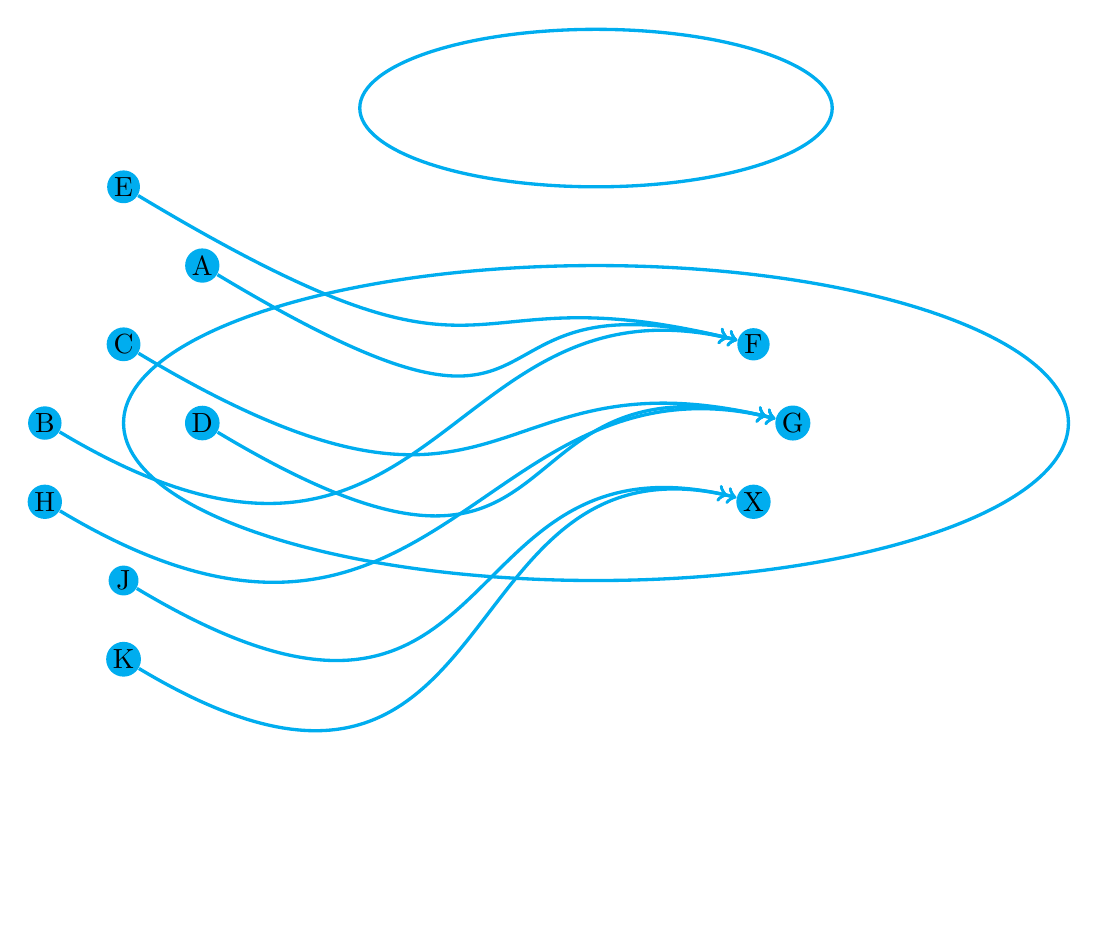
\begin{tikzpicture}

% -- center, xdim, ydim
\draw[very thick,cyan] \boundellipse{4,0}{6}{2};
\draw[very thick,cyan] \boundellipse{4,4}{3}{1};
	
  % First, define nodes
% -- points F
  
  \draw (-2,3) node[circle, inner sep=0.8pt, fill=cyan, label={{}}] (E) {E};  
  \draw (6,1) node[circle, inner sep=0.8pt, fill=cyan, label={{}}] (F) {F}; 

  \draw[very thick,cyan, ->>]  (E) .. controls +(5,-3) and +(-4,1).. (F);
  \path  ($(E)+(0,0.2)$) .. controls +(5,-3) and +(-4,1)..  ($(F)+(0,0.2)$) 
     {\foreach \i in {1,...,40} {  coordinate[pos=0.15+0.75*\i/40] (p\i) } };

  \draw (-1,2) node[circle, inner sep=0.8pt, fill=cyan, label={{}}] (A) {A};
  \draw[very thick,cyan, ->>]  (A) .. controls +(5,-3) and +(-4,1).. (F);
  \path  ($(A)+(0,0.2)$) .. controls +(5,-3) and +(-4,1)..  ($(F)+(0,0.2)$) 
     {\foreach \i in {1,...,40} {  coordinate[pos=0.15+0.75*\i/40] (p\i) } };
	
  \draw (-3,0) node[circle, inner sep=0.8pt, fill=cyan, label={{}}] (B) {B};
  \draw[very thick,cyan, ->>]  (B) .. controls +(5,-3) and +(-4,1).. (F);
  \path  ($(B)+(0,0.2)$) .. controls +(5,-3) and +(-4,1)..  ($(F)+(0,0.2)$) 
     {\foreach \i in {1,...,40} {  coordinate[pos=0.15+0.75*\i/40] (p\i) } };
	
% -- points in G

  \draw (-2,1) node[circle, inner sep=0.8pt, fill=cyan, label={{}}] (C) {C};
  \draw (6.5,0) node[circle, inner sep=0.8pt, fill=cyan, label={{}}] (G) {G};
  \draw[very thick,cyan, ->>]  (C) .. controls +(5,-3) and +(-4,1).. (G);
  \path  ($(C)+(0,0.2)$) .. controls +(5,-3) and +(-4,1)..  ($(G)+(0,0.2)$) 
     {\foreach \i in {1,...,40} {  coordinate[pos=0.15+0.75*\i/40] (p\i) } };	

\draw (-1,0) node[circle, inner sep=0.8pt, fill=cyan, label={{}}] (D) {D};	
\draw[very thick,cyan, ->>]  (D) .. controls +(5,-3) and +(-4,1).. (G);
  \path  ($(C)+(0,0.2)$) .. controls +(5,-3) and +(-4,1)..  ($(G)+(0,0.2)$) 
     {\foreach \i in {1,...,40} {  coordinate[pos=0.15+0.75*\i/40] (p\i) } };	

\draw (-3,-1) node[circle, inner sep=0.8pt, fill=cyan, label={{}}] (H) {H};	
\draw[very thick,cyan, ->>]  (H) .. controls +(5,-3) and +(-4,1).. (G);
  \path  ($(C)+(0,0.2)$) .. controls +(5,-3) and +(-4,1)..  ($(G)+(0,0.2)$) 
     {\foreach \i in {1,...,40} {  coordinate[pos=0.15+0.75*\i/40] (p\i) } };
	
% -- X
\draw (-2,-2) node[circle, inner sep=0.8pt, fill=cyan, label={{}}] (J) {J};
  \draw (6,-1) node[circle, inner sep=0.8pt, fill=cyan, label={{}}] (X) {X};
  \draw[very thick,cyan, ->>]  (J) .. controls +(5,-3) and +(-4,1).. (X);
  \path  ($(C)+(0,0.2)$) .. controls +(5,-3) and +(-4,1)..  ($(G)+(0,0.2)$) 
     {\foreach \i in {1,...,40} {  coordinate[pos=0.15+0.75*\i/40] (p\i) } };

\draw (-2,-3) node[circle, inner sep=0.8pt, fill=cyan, label={{}}] (K) {K};
\draw[very thick,cyan, ->>]  (K) .. controls +(5,-3) and +(-4,1).. (X);
  \path  ($(C)+(0,0.2)$) .. controls +(5,-3) and +(-4,1)..  ($(G)+(0,0.2)$) 
     {\foreach \i in {1,...,40} {  coordinate[pos=0.15+0.75*\i/40] (p\i) } };

%$\node [xshift=1cm,yshift=2cm] (A) at (-3,3) {Search Space};$
%$\node [xshift=1cm,yshift=2cm] (A) at (5,1) {Type System};$
	
\end{tikzpicture}
\caption{\texttt{PDB} approach} \label{fig:ss_ts}
\end{figure}
\fi

%Holte et al., (\citeyear{holte2006maximizing}) showed that search can be faster if several smaller \texttt{PDBs} are used instead of one large pattern database. In addition Domshlak et al., (\citeyear{domshlak2010max}) and Tolpin et al.,  (\citeyear{tolpin2013towards}) showed that evaluating the heuristic lazily, only when they are essential to a decision to be made in the search process, is worthy in comparison to take the maximum of the set of heuristics.
% ---
\section{Objectives}
%\subsection{Aim}
%\noindent
The objective of this dissertation is to develop algorithms for selecting a heuristic subset from a large set of heuristics with the goal of solving domain-independent planning problems. Specifically our objectives are the following. 

%\subsection{Objectives}
%\noindent

\begin{itemize}
  \item Develop a method to find a subset of heuristics from a large pool of heuristics $\zeta$ that minimizes the number of nodes expanded by A$\sp{*}$ in the process of search.
  
  \item Develop a method to find a subset of heuristics from a large pool of heuristics $\zeta$ that minimizes the A$\sp{*}$ running time.

\end{itemize}
% ---
\section{Scope, Limitations, and Delimitations}
\noindent
We implemented our method in Fast Downward \cite{helmert2006fast} and we tested our methods on the 2011 International Planning Competition (\texttt{IPC}) problem instances.

\section{Justification}
\noindent
Good results have been obtained in domain-independent planning by using heuristic search approach \cite{bonet2001planning}. The heuristic function used to guide the A$\sp{*}$ search are known to greatly affect the algorithm's running time. That is why it is important to have methods for selecting a good subset of heuristics to guide the A* search.

%We use heuristic generators in order to create a large set of heuristics and obtain heuristics to solve problems.

\section{Hypothesis}
\noindent
We test the following hypothesis:
\begin{itemize}
\item A greedy algorithm is effective for selecting a good subset of heuristics to guide the A* search.
\end{itemize}

\section{Contributions}
\noindent
The main contributions of this dissertation are:
\begin{itemize}
\item A meta-reasoning approach for selecting heuristic functions while minimizing the number of nodes generated by A$\sp{*}$.

\item A meta-reasoning approach for selecting heuristic functions while minimizing the running time of the A$\sp{*}$ search. 

\item Detailed experiments on domain-independent planning showing the strengths and weaknesses of the proposed approaches. Our experiments also show that one of our proposed approaches is able to outperform all other systems tested. 

\end{itemize}

\section{Organization}
\noindent
This dissertation is organized as follows: 
\begin{enumerate}
\item In Chapter I, the background of the dissertation is provided, which also includes the objectives and the scope definition.
\item In Chapter II we review the state-of-the-art in selection of heuristic functions.
\item In Chapter III we introduce Greedy Heuristic Selection (\texttt{GHS}). 
\item In Chapter IV compare \texttt{GHS} with other planner systems.
\item We conclude in Chapter V.
\end{enumerate}

%\clearpage
%\include{abntex2-modelo-include-comandos}
% ---

% ----------------------------------------------------------
% PARTE
% ----------------------------------------------------------
\part{Literature Review}
% ----------------------------------------------------------
%% abtex2-modelo-include-comandos.tex, v-1.9.5 laurocesar
%% Copyright 2012-2015 by abnTeX2 group at http://www.abntex.net.br/ 
%%
%% This work may be distributed and/or modified under the
%% conditions of the LaTeX Project Public License, either version 1.3
%% of this license or (at your option) any later version.
%% The latest version of this license is in
%%   http://www.latex-project.org/lppl.txt
%% and version 1.3 or later is part of all distributions of LaTeX
%% version 2005/12/01 or later.
%%
%% This work has the LPPL maintenance status `maintained'.
%% 
%% The Current Maintainer of this work is the abnTeX2 team, led
%% by Lauro César Araujo. Further information are available on 
%% http://www.abntex.net.br/
%%
%% This work consists of the files abntex2-modelo-include-comandos.tex
%% and abntex2-modelo-img-marca.pdf
%%

% ---
% Este capítulo, utilizado por diferentes exemplos do abnTeX2, ilustra o uso de
% comandos do abnTeX2 e de LaTeX.
% ---
 
\chapter{Background}\label{ch:background}
% ---
%\section{Similar Selection Systems}
% ---
\noindent
The system most similar to the one we present in this dissertation is RIDA$\sp{*}$ \cite{BarleySantiagoOver}. RIDA$\sp{*}$ also selects a subset from a pool of heuristics to guide the A$\sp{*}$ search. In RIDA$\sp{*}$ this is done by starting with an empty subset and trying subsets of size one before trying subsets of size two and so on. RIDA$\sp{*}$ stops after evaluating a fixed number of subsets. While RIDA* is able to evaluate sets of heuristics with only tens of elements, the method we propose in this dissertation is able to evaluate sets with thousands of elements.

Rayner et al., (\citeyear{raynersss13}) present an optimization procedure that is also similar to ours. In contrast with our work, Rayner et al. limited their experiments to a single objective function that sought to maximize the sum of heuristic values in the state space. Moreover, Rayner et al.'s method performs an uniform sampling of the state space to estimate the sum of heuristic values in the state space. Thus, their method is not directly applicable to domain-independent planning. In this dissertation we adapt Rayner et al.'s approach to domain-independent planning by using Stratified Sampling (\texttt{SS}) \cite{chen1992heuristic} to estimate the sum of heuristic values in the state space. Our empirical results show that \texttt{GHS} minimizing an approximation of A$\sp{*}$'s running time is able to substantially outperform Rayner et al.'s approach in domain-independent planning. 

Our meta-reasoning requires a prediction of the number of nodes expanded by A$\sp{*}$ using any given subset. One of the prediction methods we use is \texttt{SS}. Even though, \texttt{SS} produces good predictions of the Iterative-Deepening A$\sp{*}$ (IDA*)~\cite{Korf85ida} search tree, it does not produce good predictions of A$\sp{*}$'s search tree. This is because \texttt{SS} is unable to detect duplicated nodes during sampling \cite{lelis2014estimating}. Although \texttt{SS} does not produce good predictions of the number of nodes generated by A*, we show empirically that SS allows \texttt{GHS} to make good subset selections.

% ---
\section{Planning Task}
% ---

A $SAS\sp{+}$ \emph{planning task} \cite{backstrom1995complexity} is a 4 tuple $\nabla = \{V, O, I, G\}.$ \textit{V} is a set of \textit{state variables.} Each variable \textit{v} $\in$ \textit{V} is associated with a finite domain of possible $D_{\substack{v}}$. A state is an assignment of a value to every $v \in V.$ The set of possible states, denoted \textit{V}, is therefore $D_{\substack{v_{\substack{1}}}}    \times \cdots \times D_{\substack{v_{\substack{2}}}}$. \textit{O} is a set of operators, where each operator $o \in O$ is triple $\{pre_{\substack{o}} , post_{\substack{o}}, cost_{\substack{o}}\}$ specifying the preconditions, postconditions (effects), and non-negative cost of \textit{o}. $pre_{\substack{o}}\ and\ post_{\substack{o}}$ are assignments of values to subsets of variables, $V_{\substack{pre_{\substack{o}}}}\ and\ V_{\substack{post_{\substack{o}}}}$, respectively. Operator \textit{o} is applicable to state \textit{s} if \textit{s} and $pre_{\substack{o}}$ agree on the assignment of values to variables in $V_{\substack{pre_{\substack{o}}}}$. The effect of \textit{o}, when applied to \textit{s}, is to set the variables in $V_{\substack{post_{\substack{o}}}}$ to the values specified in $post_{\substack{o}}$ and to set all other variables to the value they have in $s$, resulting in a new state, which we call a \emph{child} of $s$. We define as $children(s)$ the set of child nodes of $s$. \textit{G} is the goal condition, an assignment of values to a subset of variables, $V_{\substack{G}}$. A state is a goal state if it and \textit{G} agree on the assignment of values to the variable in $V_{\substack{G}}$. \textit{I} is the initial state, and the planning task, $\nabla$, is to find an optimal (least-cost) sequence of operators leading from \textit{I} to a goal state. We denote the optimal solution cost of $\nabla$ as $C\sp{*}$. 

% ---
\section{The 8-tile-puzzle case}

The domain 8-tile-puzzle is used to illustrate a few concepts that will be helpful in the other chapters of this dissertation. The 8-tile-puzzle, illustrated in the Figure \ref{fig:8tilepuzzle_begin}, consists of a board with 8 squares named tiles numbered from 1 to 8 and one empty square. The goal of the game is to order the tiles in some order. For example: From left to right and up to bottom in the following order 1, 2, 3, 4, 5, 6, 7, 8 and empty tile. The goal can be achieved by moving the numbered tiles into the empty tile. %For this case, the goal would be reached by placing the tiles 1, 2 and 3 in the first row, and 4, 5 and 6 in the following row, and 7, 8 and empty tile in the last row.

\begin{figure}[htb]
\centering
\begin{forest}
 [\usebox\myboxa \hspace*{1.4in} \usebox\myboxb]
 $\node [xshift=-5.5cm,yshift=3.5cm] (A) at (2,0) {Initial};$
 $\node [xshift=1.5cm,yshift=3.5cm] (A) at (2,0) {Goal};$
\end{forest}
\caption{The left tile-puzzle is one possible initial distribution of tiles and the right tile-puzzle is the goal distribution of tiles. Each one represents a state.} \label{fig:8tilepuzzle_begin}
\end{figure}

Instead of using \texttt{DFS} or \texttt{BFS} that will analyze all states encountered during search to solve instances of the 8-tile-puzzle, we can obtain heuristics from the domain, which will allow search algorithms such as A* and IDA* to find a solution quicker.

\section{Heuristics}

There exist many state-space search algorithms, and one of the most important and well known is A$\sp{*}$ \cite{hart1968formal}. A$\sp{*}$ uses the $f(s) = g(s) + h(s)$ cost function to guide its search to a solution. $g(s)$ is the cost to go from the start state to state $s$, and $h(s)$ is the estimated cost to go from $s$ to the goal.

\begin{figure}[htb]
\centering
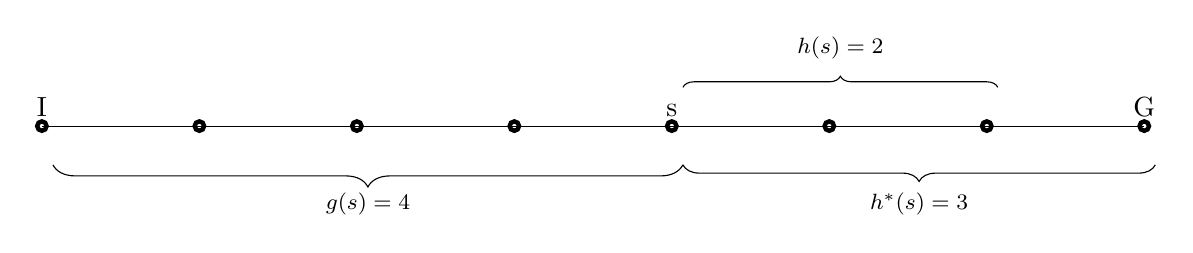
\begin{tikzpicture}
	%\draw[yshift=-1 em, ultra thick] (0,0) [point] -- (5,0) [point] -- (10,0) [point];
	\coordinate (I) at (0,0) (I) node[point=ultra thick, above] {I};
	\coordinate (I1) at (2,0) (I1) node[point=ultra thick, above] {};
	\coordinate (I2) at (4,0) (I2) node[point=ultra thick, above] {};
	\coordinate (I3) at (6,0) (I3) node[point=ultra thick, above] {};
	\coordinate (s) at (8,0) (s) node[point=ultra thick, above] {s};
	\coordinate (I4) at (10,0) (I4) node[point=ultra thick, above] {};
	\coordinate (I5) at (12,0) (I5) node[point=ultra thick, above] {};
	\coordinate (G) at (14,0) (G) node[point=ultra thick, above] {G};
	\draw (I) -- (G);	

\draw [decorate,decoration={brace,amplitude=4pt},xshift=4pt,yshift=14pt]
(8,0) -- (12,0) node [black,midway,yshift=0.5cm] 
{\footnotesize $h(s)=2$};

\draw [decorate,decoration={brace,amplitude=8pt,mirror},xshift=4pt,yshift=-14pt]
(0,0) -- (8,0) node [black,midway,yshift=-0.5cm] 
{\footnotesize $g(s)=4$};


\draw [decorate,decoration={brace,amplitude=6pt,mirror},xshift=4pt,yshift=-14pt]
(8,0) -- (14,0) node [black,midway,yshift=-0.5cm] 
{\footnotesize $h\sp{*}(s)=3$};
\end{tikzpicture}
\caption{Heuristic Search: \textit{I}: Initial state, \textit{s}: Some sate, \textit{G}: Goal state} \label{fig:searchSpace}
\end{figure}

In Figure \ref{fig:searchSpace} the optimal distance from the initial state $I$ to  the state $s$ is 4 and is represented by $g(s)$. $h\sp{*}(s) = 3$ represents the optimal distance from $s$ to the goal state $G$, and $h(s) = 2$ is the estimated cost to go from $s$ to $G$.

A heuristic is admissible if $h(s) \leq h\sp{*}(s)$ for all $s \in V$. % where $h\sp{*}(s)$ is the optimal cost of $s$. 
A heuristic is consistent iff $h(s) \leq c(s,t) + h(t)$ for all states $s$ and $t$, where $c(s,t)$ is the cost of the cheapest path from $s$ to $t$. For example, the heuristic function provided by a \texttt{PDB} \cite{culberson1998pattern} is admissible and consistent.

Given a set of admissible and consistent heuristics $\zeta = \{h_{1}, h_{2}, \dots, h_{M}\}$, the heuristic $h_{max}(s,\zeta) = $max$_{h \in \zeta} h(s)$ is also admissible and consistent. When describing our method we assume all heuristics to be consistent. We define $f_{max}(s, \zeta) = g(s) + h_{max}(s, \zeta)$, where $g(s)$ is minimal when A$\sp{*}$ using a consistent heuristic expands $s$. We call an A$\sp{*}$ search tree the tree defined by the states generated by A$\sp{*}$ using a consistent heuristic while solving a problem $\nabla$.

We now show two heuristics for the 8-tile-puzzle.

\subsection{Out-of-place Heuristic (OP)}

This heuristic counts the number of tiles that are out of the goal position. If the tile is not in its goal position, then it counts as one, otherwise it counts as zero. 

\begin{figure}[htb]
\centering
\begin{forest}
 [\usebox\myboxa]
 $\draw[->,xshift=4pt,yshift=14pt] (2,1) -- (4,1);$
 $\node [xshift=1cm,yshift=2cm] (A) at (2,0) {O.P=8};$
 \hspace*{1.8in} 
 %$\rightarrow$  
 [\usebox\myboxb] 
\end{forest}
\caption{Out of place heuristic} \label{fig:8tilepuzzle_oop}
\end{figure}

The tiles numbered with 4, 1, 2, 3, 6, 7, 5, and 8 are out of place, then each tile counts as 1 yielding a total of 8, which is heuristic value for this state.

\subsection{Manhatham Distance Heuristic (MD)}

This heuristic counts the minimum number of operations that should be applied to any tile to place it in its goal position. Let us explain this with an example: Tile 5 is located on the bottom left of the state shown on the left-hand side of Figure \ref{fig:8tilepuzzle_md}, then the minimum number of moves to get tile 5 to its goal position is 2 (either up and right or right and up), both movements equal to 2.

\begin{figure}[htb]
\centering
\begin{forest}
 [\usebox\myboxa]
 $\draw[->,xshift=4pt,yshift=14pt] (2,1) -- (4,1);$
 $\node [xshift=1cm,yshift=2cm] (A) at (2,0) {M.D=1O};$
 \hspace*{1.8in} 
 %$\rightarrow$  
 [\usebox\myboxb] 
\end{forest}
\caption{Manhatham distance heuristic} \label{fig:8tilepuzzle_md}
\end{figure}

Tile 4 requires one move to get to its goal position;
tile 1 through 7 require one move;
%tile 2 one;
%tile 3 one;
%tile 6 one;
%tile 7 one;
tiles 5 and 8 require two moves;
%tile 8 requires two;
the sum of all moves is 10, which is the MD estimate of the cost to go to this particular state. 

OP and MD are heuristics that use domain knowledge to estimate the cost to go to different states. Other methods, such as \texttt{PDBs}, do not require domain knowledge to create a heuristic function. In this dissertation we use a set of domain-independent heuristics to guide search. 

%There are methods that create heuristics without using domain knowledge, and \texttt{PDBs} are one of the most successful ways 

%Barley et al., (\citeyear{BarleySantiagoOver}) call them heuristic generators.
%
%\section{Heuristic Generators}
%
%Some heuristic generators work by creating a \texttt{PDBs}. % of the original problem space. \texttt{PDBs} are an effective way of generating heuristics. 
%One of the challenges for creating a \texttt{PDB} is to decide which abstraction to use. In our approach we use heuristic generators to generate up to thousands of \texttt{PDBs}, and then we select a subset to guide the search. 

 %\texttt{PDBs} work as follows: The search space of the problem is abstracted into a smaller state space that can be enumerated with exhaustive search. The distance of all abstracted states to the abstracted goal state are stored in a lookup table, which can be used as a heuristic function for the original state space.

\section{Using a Set of Heuristics}
A$\sp{*}$ works using a structure called \texttt{OPEN}, where in each iteration A$\sp{*}$ expands the node with the lowest cost function in \texttt{OPEN}. In Figure \ref{fig:image_h1_astar}, we have two figures wich represent the same graph, the node \texttt{a} is the initial state and the node \texttt{G} is the goal state. The problem is solved looking for the cost path starting from the initial node and finished when \texttt{G}'s node is found. Above of each node we have the heuristic value assigned by the heuristic $h_{1}$. A$\sp{*}$ add the node \texttt{a} in \texttt{OPEN} and is expanded, generating three nodes \texttt{b,c} and \texttt{d}, the node \texttt{a} is removed from \texttt{OPEN} to put it in the solution path and \texttt{b,c,d} are added to \texttt{OPEN}, A$\sp{*}$ expands the node with the lowest cost function in \texttt{OPEN}. The cost functions are $f(b)=8, f(c)=9,$ and $ f(d)=12$, then, the node \texttt{b} is chosen. In the next iteration \texttt{b} is expanded and the node \texttt{e} is generated and added to \texttt{OPEN} their cost function is calculated $f(e)=10$. For the next iteration, \texttt{c} is chosen because it has the lowest cost function and expanded and their child \texttt{f} is added to \texttt{OPEN}. The node \texttt{f} has the lowest cost function in \texttt{OPEN} because their $f(f)=9$. The \texttt{f}'s child is \texttt{G} and is added to \texttt{OPEN}. \texttt{G} is the lowest cost function and A$\sp{*}$ ask if this is the goal, if it is, then, A$\sp{*}$ stops and return the cost function of the problem which is $f(G)=9$, which is optimal.  

\begin{figure}[!htb]
\minipage{0.5\textwidth}
  \includegraphics[width=\linewidth]{images/hachefull-left}
  %\caption{A really Awesome Image}\label{fig:image1_h1_astar}
\endminipage\hfill
\minipage{0.5\textwidth}
  \includegraphics[width=\linewidth]{images/hachefullabcfG-right}
  %\caption{A really Awesome Image}\label{fig:image2_h2_astar}
\endminipage
\caption{The left figure represent the graph where above of each node is the heuristic value assigned by the heuristic $h_{1}$ and their cost to go from one node to another, the initial state is \texttt{a} and the goal state is \texttt{G}. The right figure represents the graph with the solution found by A$\sp{*}$. }\label{fig:image_h1_astar}
\end{figure}

\begin{figure}[!htb]
\minipage{0.5\textwidth}
  \includegraphics[width=\linewidth]{images/marvinh2full-left}
  %\caption{A really Awesome Image}\label{fig:image1_h1_astar}
\endminipage\hfill
\minipage{0.5\textwidth}
  \includegraphics[width=\linewidth]{images/marvinh2fulladgcfG-right}
  %\caption{A really Awesome Image}\label{fig:image2_h2_astar}
\endminipage
\caption{The left figure represent the graph where above of each node is the heuristic value assigned by the heuristic $h_{2}$ and their cost to go from one node to another, the initial state is \texttt{a} and the goal state is \texttt{G}. The right figure represents the graph with the solution found by A$\sp{*}$. }\label{fig:image_h2_astar}
\end{figure}

\begin{figure}[!htb]
\minipage{0.5\textwidth}
  \includegraphics[width=\linewidth]{images/marvinmaxfull-left}
  %\caption{A really Awesome Image}\label{fig:image1_h1_astar}
\endminipage\hfill
\minipage{0.5\textwidth}
  \includegraphics[width=\linewidth]{images/marvinmaxfullacfG-right}
  %\caption{A really Awesome Image}\label{fig:image2_h2_astar}
\endminipage
\caption{The left figure represent the graph where above of each node is the maximum heuristic value of $h_{1}$ and $h_{2}$ and their cost to go from one node to another, the initial state is \texttt{a} and the goal state is \texttt{G}. The right figure represents the graph with the solution found by A$\sp{*}$. }\label{fig:image_maxh1h2_astar}
\end{figure}

Considering that we change $h_{1}$ by another heuristic $h_2$ and for the same problem we will have the Figure \ref{fig:image_h2_astar}. The right figure shows that A$\sp{*}$ find the optimal cost path for the problem, which is 9. However, $h_{2}$ expands more nodes than $h_{1}$. Each time a node is expanded, there is a time of evaluation of the heuristic and time of generation of each node involved. If more nodes are expanded in the graph, then more time is required to solve the problem. This mean that A$\sp{*}$ with $h_{2}$ are going to last more time to find the solution than A$\sp{*}$ with $h_{1}$.

One well-know approach to take advantage of a set of heuristics $\zeta$ is to compute the maximum of all heuristics in $\zeta$. For example, given the two heuristics $h_1$ and $h_2$, the maximum of $h_1$ and $h_2$ will tend to yield a more informed heuristic than $h_1$ and $h_2$ individually. In Figure \ref{fig:image_maxh1h2_astar}, A$\sp{*}$ using the maximum of heuristics values of $h_{1}$ and $h_{2}$ expands fewer nodes than each heuristic individually. This means that the solution of the problem is found quickly.

One can easily create thousands of heuristics for a problem instance. For example, each different abstraction of a problem domain results in a different \texttt{PDB} heuristic. It is possible to prove that the maximum of all heuristics in $\zeta$ cannot be less informed than the maximum of any subset of $\zeta$. However, if $\zeta$ is too large, then the resulting heuristic obtained by taking the maximum of all heuristics in $\zeta$ can be too computationally expensive to be effective to guide search. That is why we select a subset of $\zeta$ to guide the A* search. This way we try to select the most informative heuristics in $\zeta$ while preventing the resulting maximum heuristic to be computationally expensive. 

%While taking the maximum of all heuristics in $\zeta$ will result  Using all heuristics created can 


% we need to figure it out how to take advantage of this large set of heuristics. In fact, there exist different ways to take advantage of those heuristics, however we need to take into account that if we want to use all the heuristics created by the heuristic generator, the resulting heuristic would be too expensive to guide search. This is because, the main problem involved would be the time required to evaluate all the heuristics for each node in the search tree.

%\section{Heuristic Subset}
%
%Let us suppose we have to run our meta-reasoning considering that we have a fixed amount of memory $M$. Then, one question is raised: How many heuristics our system should consider? Holte et al., (\citeyear{holte2006maximizing}) observed that maximizing over $N$ pattern databases of size $M/N$, for $N < M$, can produce a search tree size smaller than the search tree size generated by using a single pattern database of size $M$. Thus we will use heuristic generators to create a large number of heuristics to fill the amount M of memory available.
%
%Heuristic generator systems can create a large number of heuristics. Let us suppose $|\zeta| = $ 1000 heuristics were created and that our meta-reasoning for example selects $N =$ 50 heuristics. This would imply count the following number of combinations one can get from solving the combinatorial problem: $${1000\choose 50} \approx 10\sp{85} possibilities$$

In the next Chapter, we will introduce the meta-reasoning proposed for selecting a subset of $\zeta$ to guide the A* search.

\clearpage
% ---
% Capitulo de revisão de literatura
% ---
%\chapter{Lorem ipsum dolor sit amet}
% ---

% ---
%\section{Aliquam vestibulum fringilla lorem}
% ---

%\lipsum[1]

%\lipsum[2-3]

% ----------------------------------------------------------
% PARTE
% ----------------------------------------------------------
\part{Approach Proposal}
% ----------------------------------------------------------
%% abtex2-modelo-include-comandos.tex, v-1.9.5 laurocesar
%% Copyright 2012-2015 by abnTeX2 group at http://www.abntex.net.br/ 
%%
%% This work may be distributed and/or modified under the
%% conditions of the LaTeX Project Public License, either version 1.3
%% of this license or (at your option) any later version.
%% The latest version of this license is in
%%   http://www.latex-project.org/lppl.txt
%% and version 1.3 or later is part of all distributions of LaTeX
%% version 2005/12/01 or later.
%%
%% This work has the LPPL maintenance status `maintained'.
%% 
%% The Current Maintainer of this work is the abnTeX2 team, led
%% by Lauro César Araujo. Further information are available on 
%% http://www.abntex.net.br/
%%
%% This work consists of the files abntex2-modelo-include-comandos.tex
%% and abntex2-modelo-img-marca.pdf
%%

% ---
% Este capítulo, utilizado por diferentes exemplos do abnTeX2, ilustra o uso de
% comandos do abnTeX2 e de LaTeX.
% ---
 
\chapter{Meta-Reasoning for selection}\label{ch:rghs}

% ---
\section{Greedy Heuristic Selection (GHS)}
\noindent
We present a greedy algorithm selecction for approximately solving the heuristic subset selection problem while optimizing different objective functions. We consider the following general optimization problem.

\begin{equation}
\begin{split}
\textbf{minimize}_{\zeta\sp{'}\ \subseteq\ \zeta}\Psi(\zeta\sp{'}, \nabla) \\
\end{split}
\label{eq:equationmin}
\end{equation}

Where $\Psi(\zeta\sp{'},\nabla)$ is an objective function that we want to minimize using a subset of heuristics $\zeta\sp{'}$ that is selected from $\zeta$. According to Rayner et al., (\citeyear{raynersss13}) it is unlikely that there is an efficient algorithm for solving Equation \ref{eq:equationmin}.We use an algorithm based on the local search we call Greedy Heuristic Selection (\texttt{GHS}) to approximately solve Equation \ref{eq:equationmin} for different functions $\Psi$.

\begin{algorithm}
\SetKwInOut{Input}{Input}
\SetKwInOut{Output}{Output}
\Input{problem $\nabla$, set  of heuristics $\zeta$}
\Output{heuristic subset $\zeta\sp{'} \subseteq \zeta$}

$\zeta\sp{'} \leftarrow \emptyset$\\
%$i\ \leftarrow 0$\\ 
\While {$\Psi$ can be improved} {
	$h\ \leftarrow\ \argminA_{h \in \zeta}  \Psi(\zeta\sp{'} \cup \{h\}, \nabla)$\\
	$\zeta\sp{'} \leftarrow \zeta\sp{'} \cup \{h\}$\\
	%\If{$\Psi(\zeta_{i-1}\sp{'} \cup \{h\}$ can be improved}{
		%$\zeta_{i}\sp{'} \leftarrow \zeta_{i-1}\sp{'} \cup \{h\}$\\
		%$i++$\\
	%}	
} 
return $\zeta\sp{'}$
\caption{Greedy Heuristic Selection}
\label{alg:ghs_algorithm}
\end{algorithm}

Algorithm \ref{alg:ghs_algorithm} shows \texttt{GHS}. \texttt{GHS} receives as input a problem $\nabla$, a set of heuristics $\zeta$, and it returns a subset $\zeta\sp{'} \subseteq \zeta$. In each iteration \texttt{GHS} greedily selects from $\zeta$ the heuristics $h$ which will result in the largest reduction of the value $\Psi$ (line 3). \texttt{GHS} returns $\zeta\sp{'}$ once the objective function can not be improved. In other words, the algorithm will halt when adding another heuristic does not improve the objective function.

% --
\section{Approximately Minimizing Search Tree Size}
% ---
\noindent
The first objective function $\Psi$ we consider accounts for the number of expansions A$\sp{*}$ performs while solving a given planning problem. The planning problem must be solvable, this means $C\sp{*}$ can not be infinity. When solving $\nabla$ using the consistent heuristic function $h_{max}(\zeta\sp{'})$  for $\zeta\sp{'} \subseteq \zeta$, A$\sp{*}$ expands in the upper bound $J(\zeta\sp{'},\nabla)$ nodes, where

\begin{equation}
J(\zeta\sp{'},\nabla) = |\{s \in V | f_{max}(s,\zeta\sp{'}) \leq C\sp{*}\}|
\label{eq:eq_size_search_tree_1}
\end{equation}
\begin{equation}
J(\zeta\sp{'},\nabla) = |\{s \in V | h_{max}(s,\zeta\sp{'}) \leq C\sp{*} - g(s)\}|
\label{eq:eq_size_search_tree_2}
\end{equation}

We write $J(\zeta\sp{'})$ or simply $J$ instead of $J(\zeta\sp{'},\nabla)$. What's more, we assume that A$\sp{*}$ expands all nodes $s$ with $f(s) \leq C\sp{*}$ solving $\nabla$, as shown in Equation \ref{eq:eq_size_search_tree_1}. \texttt{GHS} is able to find the solutions when we use $J$ as the objective function $\Psi$.

\section{Approximately Minimizing A*'s Running Time}
\noindent
Another objective function $\Psi$ we consider accounts for the A$\sp{*}$ running time and is defined as follows. Let $T(\zeta\sp{'},\nabla)$ be an approximation to the running time of A$\sp{*}$ when using $h_{max}(\zeta\sp{'})$ for solving $\nabla$, defined as follows.

\begin{equation}
T(\zeta\sp{'}, \nabla) = J(\zeta\sp{'},\nabla) \cdot t_{h_{max}}(\zeta\sp{'})
\label{eq:eq_time_solving}
\end{equation}

where, for any heuristic function $h$, the term $t_{h}$ refers to the running time used for computing the $h-$value of any state $s$.

We assume that $t_{h}$ to be independent of $s$, which is a reasonable assumption for several heuristics such as \texttt{PDBs}.

In order to compute the running time of A$\sp{*}$ exactly we would also have to account for all nodes evaluated. Specifically, our objective function accounts for the generation time added to the heuristic evaluation time of all nodes generated, not only nodes expanded. In this way, $T(\zeta\sp{'},\nabla)$ is reasonable approximation for A$\sp{*}$'s running time for the heuristic subset selection problem.\\

\section{Estimating Tree Size and Running Time}
In  practice \texttt{GHS} used approximations models of $J,T,$ and $T\sp{'}$ instead of their exact values. This is because computing $J,T,$ and $T\sp{'}$ exactly would require solving $\nabla$, and this is what we obviously want to avoid. We denote the approximations of $J$ as \textit{\^{J}}, and since both $T$ and $T\sp{'}$ model A$\sp{*}$'s running time, we denote the approximation for both as \textit{\^{T}}.

We use the Culprit Sampler (\texttt{CS}) introduced by Barley et al., (\citeyear{BarleySantiagoOver}) and the Stratified Sampling (\texttt{SS}) algorithm introduced by Chen, (\citeyear{chen1992heuristic}) for computing \textit{\^{J}} and \textit{\^{T}}. Each of the two algorithms has its strengths and weaknesses, which we explore in the experimental Chapter.

Both \texttt{CS} and \texttt{SS} must be able to quickly estimate the values of \textit{\^{J}}$(\zeta\sp{'})$ and \textit{\^{T}}$(\zeta\sp{'})$ for any subset $\zeta\sp{'}$ of $\zeta$ so they can be used in \texttt{GHS}'s optimization process.

\section{Culprit Sampler (CS)}
\noindent
\texttt{CS} runs a time$-$bounded A$\sp{*}$ search while sampling $f-culprits$ and $b-culprits$ to estimate the values of \textit{\^{J}} and \textit{\^{T}}.

\begin{definition}(f-culprit)
Let $\zeta = \{h_{1}, h_{2},...,h_{M}\}$ be a set of heuristics. The f$-$culprit of a node n in an A$\sp{*}$ search tree is defined as the tuple F(n) = $\left\langle f_{1}(n), f_{2}(n),...,f_{M}(n)  \right\rangle$, where $f_{i}(n) = g(n)+h_{i}(n)$. For any n$-$tuple F, the counter $C_{F}$ denotes the number of nodes n in the tree with F(n) = F.
\label{def:def_fculprits}
\end{definition}

\begin{definition}(b-culprit)
Let $\zeta = \{h_{1}, h_{2},...,h_{M}\}$ be a set of heuristics and b a lower bound on the solution cost $\nabla$. The b$-$culprit of a node n in an A$\sp{*}$ search tree is defined as the tuple $B(n) = \left\langle y_{1}(n), y_{2}(n),...,y_{M}(n)\right\rangle$, where $y_{i}(n) = 1$ if g(n) + $h_{i}(n) \leq b$ and $y_{i}(n) = 0$, otherwise.  For any binary n$-$tuple B, the counter $C_{B}$ denotes the number of nodes n in the tree with B(n) = B.
\label{def:def_bculprits}
\end{definition}

\texttt{CS} works by running an A$\sp{*}$ search bounded by a user$-$specified time limit. Then, \texttt{CS} compresses the information obtained in the A$\sp{*}$ search (\textsf{i.e.,} the $f-$values of all nodes expanded according to all heuristics $h$ in $\zeta$) in b$-$culprits, which are later used for computing \textit{\^{J}}. The f$-$culprits are generated as an intermediate step for computing the b$-$culprits, as we explain below. The maximum number of f$-$culprits and b$-$culprits in an A$\sp{*}$ search tree is equal to the number of nodes in the tree expanded by the time$-$bounded A$\sp{*}$ search. However, in practice the number of f$-$culprits is usually much lower than the number of nodes in the tree. Moreover, in practice, the total number of different b$-$culprits tends to be even lower than the total number of f$-$culprits. Given a planning problem $\nabla$ and a set of heuristics $\zeta$, \texttt{CS} samples the A$\sp{*}$ search tree as follows.

\begin{enumerate}
    \item[1.-] \texttt{CS} runs A$\sp{*}$ using $h_{min}(s,\zeta) = min_{h \in \zeta}h(s)$ until reaching a user$-$specified time limit. A$\sp{*}$ using $h_{min}$ expands node $n$ if it were to expand $n$ while using any of the heuristics in $\zeta$ individually. For each node $n$ expanded in this time$-$bounded search we store $n$'s f$-$culprit and its counter.
    \item[2.-] Let $f_{maxmin}$ be the largest $f-$value according to $h_{min}$ encountered in the time$-$bounded A$\sp{*}$ search described above. We now compute the set $\mathbb{B}$ of b$-$culprits and their counters based on the f$-$culprits and on the value of $f_{maxmin}$. This is done by iterating over all f$-$culprits once.

\end{enumerate}
    
The process described above is performed only once \texttt{GHS}'s execution. The value of \textit{\^{J}}$(\zeta\sp{'},\nabla)$ for any subset $\zeta\sp{'}$ of $\zeta$ if then computed by iterating over all b$-$culprits \textbf{B} and summing up the relevant values of $C_{B}$. The relevant values of $C_{B}$ represent the number of nodes A$\sp{*}$ would expand in a search bounded by $b$ if using $h_{max}(\zeta\sp{'})$. This computation can be written as follows.

\begin{equation}
\textit{\^{J}}(\zeta\sp{'},\nabla) = \sum_{\mathbb{B} \in B}W(B)
\label{eq:eq_comp_w}
\end{equation}

Where $W(B)$ is 0 if there is a heuristic in $\zeta\sp{'}$ whose $y$-value in $B$ is zero (\textsf{i.e.,} there is a heuristic in $\zeta\sp{'}$ that prunes all nodes compressed into $B$), and $C_{B}$ otherwise. If the time$-$bounded A$\sp{*}$ search with $h_{min}$ expands all nodes $n$ with $f(n) \leq C\sp{*}$, then \textit{\^{J}}$=J$. In practice, however, our estimate \textit{\^{J}} will tend to be much lower than $J$.

The value of \textit{\^{T}} is computed by multiplying \textit{\^{J}} by the sum of the evaluation time of each heuristic in $\zeta\sp{'}$. The evaluation time of the heuristics in $\zeta\sp{'}$ is measured in a separate process, before executing \texttt{CS}, by sampling a small number of nodes from $\nabla$'s start state.

\section{Stratified Sampling (SS)}
Chen, (\citeyear{chen1992heuristic}) presented a method for estimating the search tree size of backtracking search algorithms by using a stratification of the search tree to guide its sampling. We define Chen’s stratification as a type system.

\begin{figure}[htb]
\centering 
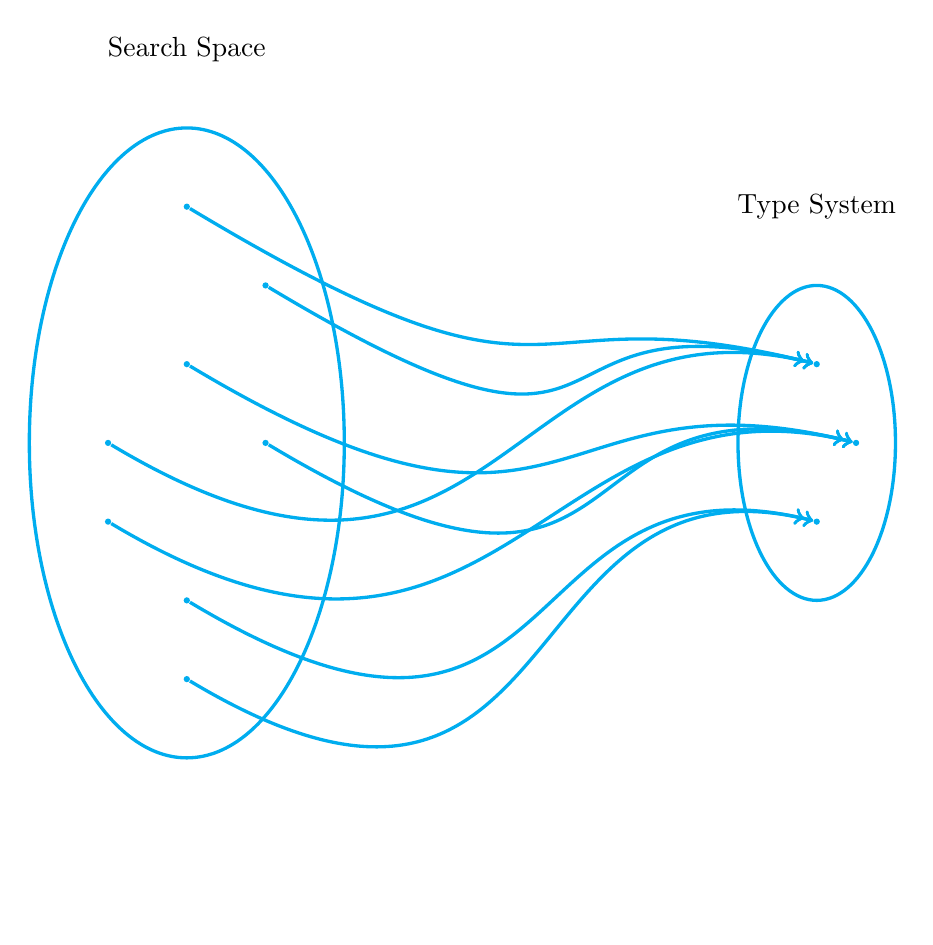
\begin{tikzpicture}

% -- center, xdim, ydim
\draw[very thick,cyan] \boundellipse{-2,0}{2}{4};
\draw[very thick,cyan] \boundellipse{6,0}{1}{2};
	
  % First, define nodes
% -- points F  
  
  \draw (-2,3) node[circle, inner sep=0.8pt, fill=cyan, label={{}}] (E) {};  
  \draw (6,1) node[circle, inner sep=0.8pt, fill=cyan, label={{}}] (F) {}; 

  \draw[very thick,cyan, ->>]  (E) .. controls +(5,-3) and +(-4,1).. (F);
  \path  ($(E)+(0,0.2)$) .. controls +(5,-3) and +(-4,1)..  ($(F)+(0,0.2)$) 
     {\foreach \i in {1,...,40} {  coordinate[pos=0.15+0.75*\i/40] (p\i) } };

  \draw (-1,2) node[circle, inner sep=0.8pt, fill=cyan, label={{}}] (A) {};
  \draw[very thick,cyan, ->>]  (A) .. controls +(5,-3) and +(-4,1).. (F);
  \path  ($(A)+(0,0.2)$) .. controls +(5,-3) and +(-4,1)..  ($(F)+(0,0.2)$) 
     {\foreach \i in {1,...,40} {  coordinate[pos=0.15+0.75*\i/40] (p\i) } };
	
  \draw (-3,0) node[circle, inner sep=0.8pt, fill=cyan, label={{}}] (B) {};
  \draw[very thick,cyan, ->>]  (B) .. controls +(5,-3) and +(-4,1).. (F);
  \path  ($(B)+(0,0.2)$) .. controls +(5,-3) and +(-4,1)..  ($(F)+(0,0.2)$) 
     {\foreach \i in {1,...,40} {  coordinate[pos=0.15+0.75*\i/40] (p\i) } };
	
% -- points in G

  \draw (-2,1) node[circle, inner sep=0.8pt, fill=cyan, label={{}}] (C) {};
  \draw (6.5,0) node[circle, inner sep=0.8pt, fill=cyan, label={{}}] (G) {};
  \draw[very thick,cyan, ->>]  (C) .. controls +(5,-3) and +(-4,1).. (G);
  \path  ($(C)+(0,0.2)$) .. controls +(5,-3) and +(-4,1)..  ($(G)+(0,0.2)$) 
     {\foreach \i in {1,...,40} {  coordinate[pos=0.15+0.75*\i/40] (p\i) } };	

\draw (-1,0) node[circle, inner sep=0.8pt, fill=cyan, label={{}}] (D) {};	
\draw[very thick,cyan, ->>]  (D) .. controls +(5,-3) and +(-4,1).. (G);
  \path  ($(C)+(0,0.2)$) .. controls +(5,-3) and +(-4,1)..  ($(G)+(0,0.2)$) 
     {\foreach \i in {1,...,40} {  coordinate[pos=0.15+0.75*\i/40] (p\i) } };	

\draw (-3,-1) node[circle, inner sep=0.8pt, fill=cyan, label={{}}] (H) {};	
\draw[very thick,cyan, ->>]  (H) .. controls +(5,-3) and +(-4,1).. (G);
  \path  ($(C)+(0,0.2)$) .. controls +(5,-3) and +(-4,1)..  ($(G)+(0,0.2)$) 
     {\foreach \i in {1,...,40} {  coordinate[pos=0.15+0.75*\i/40] (p\i) } };
	
% -- X
\draw (-2,-2) node[circle, inner sep=0.8pt, fill=cyan, label={{}}] (J) {};
  \draw (6,-1) node[circle, inner sep=0.8pt, fill=cyan, label={{}}] (X) {};
  \draw[very thick,cyan, ->>]  (J) .. controls +(5,-3) and +(-4,1).. (X);
  \path  ($(C)+(0,0.2)$) .. controls +(5,-3) and +(-4,1)..  ($(G)+(0,0.2)$) 
     {\foreach \i in {1,...,40} {  coordinate[pos=0.15+0.75*\i/40] (p\i) } };

\draw (-2,-3) node[circle, inner sep=0.8pt, fill=cyan, label={{}}] (K) {};
\draw[very thick,cyan, ->>]  (K) .. controls +(5,-3) and +(-4,1).. (X);
  \path  ($(C)+(0,0.2)$) .. controls +(5,-3) and +(-4,1)..  ($(G)+(0,0.2)$) 
     {\foreach \i in {1,...,40} {  coordinate[pos=0.15+0.75*\i/40] (p\i) } };

$\node [xshift=1cm,yshift=2cm] (A) at (-3,3) {Search Space};$

$\node [xshift=1cm,yshift=2cm] (A) at (5,1) {Type System};$
	
\end{tikzpicture}
\caption{Type system and the search space representation.} \label{fig:ss_ts}
\end{figure}

\subsection{Type System}
The type system is calculated based of any property of each node in the search space. In addition, this new search space that is created with the types is called partition of the search space and nodes are going to have the same type if they have the same $f$-value. Lelis et al., (\citeyear{lelis2013predicting}). In the Figure \ref{fig:ss_ts} we can see that the type system is a partition of the type system.

\iffalse
A common mistake about type system is to think that it is an abstraction of the state$-$space. Prieditis, (\citeyear{Prieditis93}) defines a state$-$space abstraction as a simplified version of the problem where:
\begin{itemize}
\item The cost of the least$-$cost path between two abstracted states must less than or equal to the cost of the least$-$cost path between the corresponding two states in the original state$-$space.
\item Goal states in the original state$-$space must be goal states in the abstracted state$-$space.
\end{itemize}

The difference between state-space abstractions and type system is that the last one does not have the two requeriments mentioned above. Also, there is not relation between types to argue that the type system can be represented as a graph. Furthermore, the relation between type system and abstractions is that type system can not necessarily used as abstractions, and abstraction always can be used as a type system Prieditis, (\citeyear{Prieditis93}).
\fi

\begin{definition}{Type System}
Let S = (N,E) be a search tree, where N is its set of nodes and  for each n $\in$ N, $\{n\sp{'}|(n,n\sp{'})\ \in\ E \}$ is n's set of child nodes. $TS = \{t_{1},...,t_{k} \}$ is a type system for S if it is a disjoint partitioning of N. If $n\ \in\ N$ and $t\ \in\ TS$ with $n\ \in\ t$, we write $TS(n) = t$.
\end{definition}

According to Lelis et al., (\citeyear{lelis2013predicting}), \texttt{SS} is a general method for approximating any function of the form $\varphi = \sum_{n \in S}z(n)$, where $z$ is any function assigning a numerical value to a node.  $\varphi$ represents a numerical property of the search tree rooted at $n\sp{*}$. For instance, if $z(n)=1$ for all $n \in S$, then $\varphi$ is the size of the tree. Instead of traversing the entire tree and summing all $z-$values, \texttt{SS} assumes subtrees rooted at nodes of the same type will have equal values of $\varphi$ and only one node of each type, chosen randomly, is expanded. This is the key to $\texttt{SS}$'s efficiency since the search trees of practical interest have far too many nodes to be examined exhaustively. Given a search tree $S$ and a type system $TS$, \texttt{SS} estimates $\varphi$ as follows. First, it samples the tree and returns a set $A$ of $representative-weight$ pairs, with one such pair for every unique type seen during sampling. In the pair $\left\langle s,w \right\rangle$ in $A$ for type $t \in TS$, $n$ is the unique node of type $t$ that was expanded during search and $w$ is an estimate of the number of nodes type $t$ in the tree. $\varphi$ is then approximated by $\hat{\varphi}$, defined as, $\hat{\varphi} =  \sum_{\left\langle s,w \right\rangle \in A}w \times z(n)$. 

By making $z(n) = 1$ for all $n \in S$ \texttt{SS} prooduces an estimate $\hat{J}$ of $J$. Similarly to our approach with \texttt{CS}, we obtain $\hat{T}$ by multiplying $\hat{J}$ by the heuristic evaluation time.


\begin{algorithm}
\SetKwInOut{Input}{Input}
\SetKwInOut{Output}{Output}
\Input{root $n\sp{*}$ of a tree and a type system $TS$, upper bound $d$, heuristic function $h$}
\Output{an array of sets $A$, where $A[i]$ is the set of (node, weight) pairs $<s,w>$ for the nodes $n$ expanded at level $i$.}

$A[0] \leftarrow \{\left\langle  s\sp{*},1 \right\rangle \}$

$i \leftarrow 0$

\While{A[i] is not empty} {
	\For{each element $\left\langle s,w \right\rangle$ in $A[i]$} {
		\For{each child $\hat{n}$ of n} {
			\If{$g(\hat{n}) + h(\hat{n}) \leq d$} {
				\If{$A[i+1]$ contains an element $\left\langle n\sp{'}, w\sp{'} \right\rangle$ with $TS(n\sp{'}) = TS(\hat{n})$} {
				$w\sp{'} \leftarrow w\sp{'} + w$\\ 
				with probability $w/w\sp{'}$, replace $\left\langle n\sp{'}, w\sp{'} \right\rangle$ in $A[i+1]$ by $\left\langle \hat{n},w\sp{'} \right\rangle$
				} \Else {	
					insert new element $\left\langle \hat{n},w \right\rangle$	 in $A[i+1]$
				}
			}
		}
	}
	$i \leftarrow i + 1$
}
\caption{SS, a single probe}
\label{alg:ss_algorithm}
\end{algorithm}

In \texttt{SS} the types are required to be partially ordered: a node's type must be strictly greater than the type of its parent. This can be guaranteed by adding the depth of a node to the type system and then sorting the types lexicographically. That is why in our implementation of \texttt{SS} types at one level are treated separately from types at another level by the division of $A$ into groups $A[i]$, where $A[i]$ is the set of representative$-$weight pairs for the types encountered at level $i$. If the same type occurs on differente levels the occurrences will be treated as if they were different types $-$ the depth of search is implicitly included into all of our type systems.

Algorithm \ref{alg:ss_algorithm} shows \texttt{SS} in detail. Representative nodes from $A[i]$ are expanded to get representative nodes for $A[i+1]$ as follows. $A[0]$ is initialized to contain only the root of the search tree to be probed, with weight 1 (Line 1). In each iteration (Lines 4 through 11), all nodes in $A[i]$ are expanded. The children of each node in $A[i]$ are considered for inclusion in $A[i+1]$ if their $f-$value do not exceed an upper bound $d$ provided as input to \texttt{SS}. If a child $\hat{n}$ has a type $t$ that is already represented in $A[i+1]$ by another node $n\sp{'}$, then a $merge$ action on $\hat{n}$ and $n\sp{'}$ is performed. In a merge action we increase the weight in the corresponding representative$-$weight pair of type $t$ by the weight $w(n)$ of $\hat{n}$'s parent $n$ (from level $i$) since there were $w(n)$ nodes at level $i$ that are assumed to have children of type $t$ at level $i+1$. $\hat{n}$ will replace $n\sp{'}$ according to the probability shown in Line 9. Chen, (\citeyear{chen1992heuristic}) proved that this probability reduces the variance of the estimation. Once all the states in $A[i]$ are expanded, we move to the next iteration.

One run of the \texttt{SS} algorithm is called a $probe$. Chen,  (\citeyear{chen1992heuristic}) proved that the expected value of $\hat{\varphi}$ converges to $\varphi$ in the limit as the number of probes goes to infinity. As Lelis et al., (\citeyear{lelis2014estimating}), \texttt{SS} is not able to detect duplicated nodes in its sampling process. As a result, since A$\sp{*}$ does not expanded duplicates, \texttt{SS} usually overestimates the actual number of nodes A$\sp{*}$ expands. Thus, in the limit, as the number of probes grows large, \texttt{SS}'s prediction converges to a number which  is likely to overestimate the A$\sp{*}$ search tree size. We test empirically whether \texttt{SS} is able to allow \texttt{GHS} to make good subset selects despite being unable to detect duplicated nodes during sampling.

Similarly to \texttt{CS}, we also define a time$-$limit to run \texttt{SS}. We use \texttt{SS} with an iterative$-$deepening approach in order to ensure an estimate of $\hat{J}$ and $\hat{T}$ before reaching the time limit. We set the upper bound $d$ to the heuristic value of the start state and, after performing $p$ probes, if there is still time, we increase $d$ to twice its previous value. The values of $\hat{J}$ and $\hat{T}$ is given by the prediction produced for the last $d-$value in which \texttt{SS} was able to perform all $p$ probes.

\texttt{SS} must also be able to estimate the values of $\hat{J}(\zeta\sp{'})$ and $\hat{T}(\zeta\sp{'})$ for any subset $\zeta\sp{'}$ of $\zeta$. This is achieved by using \texttt{SS} to estimate b$-$culprits (See Definition \ref{def:def_bculprits}) instead of the search tree size directly. Similarly to \texttt{CS, SS} used $h_{min}$ of the heuristics in $\zeta$ to decide when to prune a node (See Line 6 of Algorithm \ref{alg:ss_algorithm}) while sampling. This ensures that \texttt{SS} expands a node $n$ if A$\sp{*}$ employing at least one of the heuristics in $\zeta$ would expand $n$ according to bound $d$. The $C_{B}$ counter of each b$-$culprit $B$ encountered during $SS$'s probe is given by,

\begin{equation}
C_{B} = \sum_{\left\langle n,w \right\rangle \in A \wedge B(n) = B}w
\label{eq:eq_CB}
\end{equation}

We recall that to compute $B(n)$ for node $n$ one needs to define a bound $b$. Here we use the bound $d$ used by \texttt{SS}. The average value of $C_{B}$ across $p$ probes is used to predict the search tree size for a given subset $\zeta\sp{'}$. As explained for \texttt{CS}, this can be done by traversing over all b$-$culprits once.

\if false

\section{8-tile-puzzle Case Using type system}
\noindent
In this dissertation we use type system based only in heuristics.\cite{lelis2013predicting} use the type system where two nodes have the same type if they have the same heuristic value.

\begin{figure}[htb]
\centering
\begin{forest}
 [\usebox\myboxc \hspace*{1.4in} \usebox\myboxb]
\end{forest}
\caption{The heuristic value is the position of the empty tile in a specific state.} \label{fig:type_system}
\end{figure}

Let's explain how type system works through an example. The problem of 8-tile-puzzle in the Figure \ref{fig:type_system}, the center tile is labeled with the letter \texttt{M}, the corners labeled with \texttt{C} and the mediums with \texttt{E}. For this problem, we can define the type system based on the position of the empty tile regarding the position of the empty tile in the goal state. For this case, two nodes $n$ and $n\sp{'}$ would be of the same type if $n$ and $n\sp{'}$ have the empty tile with the same letter and with the same distance to the empty tile of the goal state.

In the Figure \ref{fig:empty_space_ts}, each row represent a type. The first board shows the empty tile in the center with distance to the empty tile in the goal state equal to 2. The shortest path to get to the empty tile in the goal state would be doing: down$-$left or right$-$down. Which both moves represent the same cost. Then, the type would be (2,\texttt{M}). In the next board, the empty tile is in the left top, and use the letter \texttt{C}. The minimum distance is 4 because to get the goal empty tile is necessary to do: down$-$down$-$right$-$right or right$-$right$-$down$-$down, etc. So the type would be (4, \texttt{C}). In the next board, there are two tiles that have the same type, because both have the same letter \texttt{M} with distance equal to 3. Then, both have the type (3,E). The fourth row have two boards with the same type, because both have the same letter \texttt{C} with distance equal to 2. Then, both have the type (2, \texttt{C}). The fifth row have two boards with the same type, because both have the same letter \texttt{E} with distance equal to 1. Then, both have the type (1, \texttt{E}). In the last row the empty tile is in the goal empty tile. So, the distance is zero and the letter is \texttt{C}. The type would be (0, \texttt{C}).

% print types
\begin{figure}[htb]
\centering
\begin{forest}
 [\usebox\myboxcenter]
 $\node [xshift=1cm,yshift=2cm] (A) at (2,0) {(2, M)};$
\end{forest}

\begin{forest}
 [\usebox\myboxcornerone]
 $\node [xshift=1cm,yshift=2cm] (A) at (2,0) {(4, C)};$
\end{forest}

\begin{forest}
 [\usebox\myboxmediumleft \hspace*{0.2in} \usebox\myboxmediumup]
 $\node [xshift=1cm,yshift=2cm] (A) at (4,0) {(3, E)};$
\end{forest}

\begin{forest}
 [\usebox\myboxcornerthree \hspace*{0.2in} \usebox\myboxcornertwo]
 $\node [xshift=1cm,yshift=2cm] (A) at (4,0) {(2, C)};$
\end{forest}

\begin{forest}
 [\usebox\myboxmediumdown \hspace*{0.2in} \usebox\myboxmediumright]
 $\node [xshift=1cm,yshift=2cm] (A) at (4,0) {(1, E)};$
\end{forest}

\begin{forest}
 [\usebox\myboxcornerfour]
 $\node [xshift=1cm,yshift=2cm] (A) at (2,0) {(0, C)};$
\end{forest}
\caption{Each row has one or two states that represent the same type.} \label{fig:empty_space_ts}
\end{figure}

\fi

\section{SS step by step}
\noindent
% -- Explaining Stratified Sampling
In the Figure \ref{fig:ts_search_tree}, we can see how type system works. In this dissertation we use type system based only in heuristics. Lelis et al., (\citeyear{lelis2013predicting}) use the type system where two nodes have the same type if they have the same heuristic value. 

In the Level 1, we have the root node, the $w$ initialized with one. Let's suppose that three nodes are generated by the root node in the Level 2. The nodes in the Level 2 have the following types: red, blue and red from left to right respectively, and each node receive the same $w$ of the father. In the Level 2 we apply \texttt{SS}'s assumption, two nodes in the same level that have the same type (The same color) root subtrees of the same size and only one node of each type must be chosen randomly to be expanded. There are two nodes with type red in Level 2. In that way, we choose randomly one of them. Let's suppose we choose the right red node. Then, we have to update the number of nodes with the type red using the $w$, both red node types have $w=1$, then we sum the $w$ and the new $w=2$. As a result, in the Level 2 we will have two nodes of red type and one node with blue type.

\begin{figure}[htb]
\centering
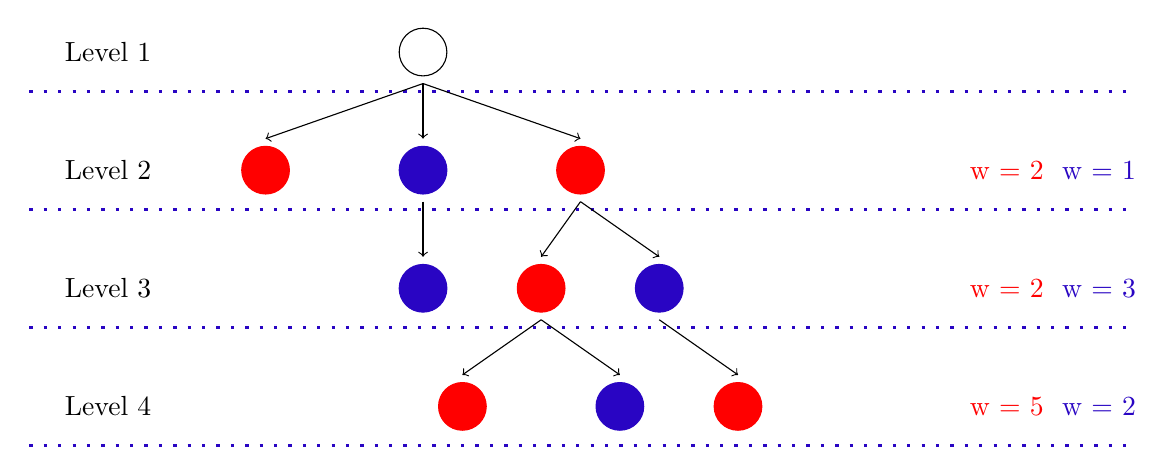
\begin{tikzpicture}

\draw[very thick,blue,loosely dotted] (-2,0) -- (12,0);
\draw[very thick,blue,loosely dotted] (-2,-1.5) -- (12,-1.5);
\draw[very thick,blue,loosely dotted] (-2,-3) -- (12,-3);
\draw[very thick,blue,loosely dotted] (-2,-4.5) -- (12,-4.5);

\node [xshift=1cm,yshift=2cm] (A) at (-2,-1.5) {Level 1};
\node [xshift=1cm,yshift=2cm] (A) at (-2,-3) {Level 2};
\node [xshift=1cm,yshift=2cm] (A) at (-2,-4.5) {Level 3};
\node [xshift=1cm,yshift=2cm] (A) at (-2,-6) {Level 4};

% -- level 1
\draw[black,fill=white] (3,0.5) circle (2ex);

% -- level 2
\draw[red,fill=red] (1,-1) circle (2ex);
\draw[blue,fill=blue] (3,-1) circle (2ex);
\draw[red,fill=red] (5,-1) circle (2ex);

% -- level 3
\draw[blue,fill=blue] (3,-2.5) circle (2ex);
\draw[red,fill=red] (4.5,-2.5) circle (2ex);
\draw[blue,fill=blue] (6,-2.5) circle (2ex);

% -- level 4
\draw[red,fill=red] (3.5,-4) circle (2ex);
\draw[blue,fill=blue] (5.5,-4) circle (2ex);
\draw[red,fill=red] (7,-4) circle (2ex);

% -- draw arrows
\draw[->] (3,0.1) -- (1,-0.6);
\draw[->] (3,0.1) -- (3,-0.6);
\draw[->] (3,0.1) -- (5,-0.6);

\draw[->] (3,-1.4) -- (3,-2.1);

\draw[->] (5,-1.4) -- (4.5,-2.1);
\draw[->] (5,-1.4) -- (6,-2.1);

\draw[->] (4.5,-2.9) -- (3.5,-3.6);
\draw[->] (4.5,-2.9) -- (5.5,-3.6);

\draw[->] (6,-2.9) -- (7,-3.6);

\node [xshift=1cm,yshift=2cm] (A) at (10,-3) {\textcolor{red}{w = 2 } \textcolor{blue}{w = 1}};
\node [xshift=1cm,yshift=2cm] (A) at (10,-4.5) {\textcolor{red}{w = 2 } \textcolor{blue}{w = 3}};
\node [xshift=1cm,yshift=2cm] (A) at (10,-6) {\textcolor{red}{w = 5 } \textcolor{blue}{w = 2}};
\end{tikzpicture}
\caption{Search tree using Type System} \label{fig:ts_search_tree}
\end{figure}

Let's suppose that nodes in Level 2 are expanded. The blue node expands one node of type blue and the red node expands two nodes of type red and blue. The question here is how many nodes are generated in the Level 3. The answer is: $1 \times \textcolor{blue}{blue} + 2 \times \textcolor{red}{red} + 2 \times \textcolor{blue}{blue}$. So, in the Level 3 we will have 2 nodes of type red and 3 nodes of type blue.

In the Level 3 the $w$ of the node blue would have the same $w$ of the father. The father has $w = 1$, then the child has $w = 1$. The $w$ of the red type and blue type would be 2. Once the $w$ has been updated for each node in the Level 3 we apply the \texttt{SS}'s assumption again. There are two nodes with type blue. Then, we choose randomly one of them and update their $w$. Let's choose the right blue type and the updated $w$ would be 3 because 1 from the left blue type plus the 2 from the right blue type.

When nodes in the Level 3 are expanded. They are expanded in the following way: The red node expands two nodes of types red and blue and the blue node expands one of type red. How many nodes would be generated at Level 4, then? The answer is: $2 \times \textcolor{red}{red} + 3 \times \textcolor{red}{red} + 2 \times \textcolor{blue}{blue}$. Therefore, in the Level 4, we will have five nodes of type red and two nodes of type blue.

Finally, the number of nodes expanded in the search tree is obtained summing all $w$ plus one (The root node). As a result, the number of nodes expanded in the search tree would be $ 15 + 1 = 16$.

\clearpage
% ---

% PARTE
% ----------------------------------------------------------
\part{Empirical Evaluation}
% ----------------------------------------------------------
%% abtex2-modelo-include-comandos.tex, v-1.9.5 laurocesar
%% Copyright 2012-2015 by abnTeX2 group at http://www.abntex.net.br/ 
%%
%% This work may be distributed and/or modified under the
%% conditions of the LaTeX Project Public License, either version 1.3
%% of this license or (at your option) any later version.
%% The latest version of this license is in
%%   http://www.latex-project.org/lppl.txt
%% and version 1.3 or later is part of all distributions of LaTeX
%% version 2005/12/01 or later.
%%
%% This work has the LPPL maintenance status `maintained'.
%% 
%% The Current Maintainer of this work is the abnTeX2 team, led
%% by Lauro César Araujo. Further information are available on 
%% http://www.abntex.net.br/
%%
%% This work consists of the files abntex2-modelo-include-comandos.tex
%% and abntex2-modelo-img-marca.pdf
%%

% ---
% Este capítulo, utilizado por diferentes exemplos do abnTeX2, ilustra o uso de
% comandos do abnTeX2 e de LaTeX.
% ---

\externaldocument[I-]{chapter03}

\chapter{Empirical Evaluation}\label{ch:empirical_evaluation}
\noindent
The practical effectiveness of \texttt{GHS} depends on its ability of finding good approximations $\hat{J}$ and $\hat{T}$. In order to verify its practical effectiveness, we have implemented \texttt{GHS} in Fast Downward (Helmert, \citeyear{helmert2006fast}) and tested the A$\sp{*}$ performance using subsets of heuristics selected by \texttt{GHS} while minimizing different objective funcions.

We run two sets of experiments. In the first set we verify whether the approximations $\hat{J}$ and $\hat{T}$ provided by \texttt{CS} and \texttt{SS} allow \texttt{GHS} selects good subset selections for A$\sp{*}$ search tree size and running time. In the second set of experiments we test the effectiveness of \texttt{GHS} by measuring the total number of problem instances solved by A$\sp{*}$ using a heuristic subset selected by \texttt{GHS}.

\texttt{GHS} is executed up to adding another heuristic does not improve the objective function. In each iteration \texttt{GHS} greedily selects from $\zeta$ the heuristic $h$ which will result in the largest reduction of the value of the objective function $\Psi$. We can't control the size of the resulting subset because \texttt{GHS} stops if adding another heuristic $h$ to the $\zeta\sp{'}$ does not improve the objective function and returns the current subset $\zeta\sp{'}$.

% Please add the following required packages to your document preamble:
% \usepackage{multirow}
\begin{table}[]
\centering
\caption{Ratios of the number of nodes generated using $h_{max}(\zeta\sp{'})$ to the number of nodes generated using $h_{max}(\zeta)$}
\begin{tabular}{lrrrrrr}
\hline
\multirow{2}{*}{Domain} & \multicolumn{2}{c}{\texttt{SS}} & \multicolumn{2}{c}{\texttt{CS}}   & \multirow{2}{*}{|$\zeta$|} & \multirow{2}{*}{n} \\ \cline{2-5}
                        & Ratio    & |$\zeta\sp{'}$|   & Ratio  & |$\zeta\sp{'}$| &                            &                    \\ \hline
Barman                  & 1.11     & 17.70       & 1.50   & 30.25           & 5168.50                    & 20                 \\
Elevators               & 11.50     & 2.00       & 1.03   & 21.00           & 168.00                     & 1                  \\
Floortile               & 1.02     & 43.07       & 1.01   & 42.35           & 151.28                     & 14                 \\
Openstacks              & 1.00     & 1.00        & 1.00   & 1.00            & 390.69                     & 13                 \\
Parking                 & 1.00     & 5.52        & 1.01   & 7.26            & 21.73                      & 19                 \\
Pegsol                  & 1.00     & 31.00       & 1.00   & 57.00           & 90.00                      & 2                  \\
Scanalyzer              & 1.22     & 30.57       & 1.56   & 19.42           & 72.85                      & 7                  \\
Tidybot                 & 1.00     & 2.35        & 1.00   & 8.58            & 3400.17                    & 17                 \\
Transport               & 1.00     & 14.70        & 1.02   & 14.30           & 171.7                     & 10                  \\
Visitall                & 1.02     & 99.33       & 1.18   & 48.66           & 256.33                     & 3                  \\
Woodworking             & 32.42     & 3.00       & 199.65 & 5.00           & 1289.00                     & 5                  \\ \hline
\end{tabular}
\label{tb_one}
\end{table}

\iffalse
In all our experiments we use a type system that assigned the same type for a node with the same $f-$value. Such a type system has shown to be effective in guiding \texttt{SS} to produce accurate tree size predictions in other application domains Lelis et al., (\citeyear{lelis2013predicting}), Lelis et al., (\citeyear{lelis2014memory}).
\fi

We ran our experiments on the 2011 International Planning Competition (\texttt{IPC}) instances. We used the 2011 instances instead of the 2014 instances because the former do not have problems with conditional effects, which are currently not handled by \textbf{PDB} heuristics. All experiments are run on $2.67$ GHz machines with 4GB, and are limited to 1,800 seconds of running time.

% ---
\section{Empirical Evaluation of $\hat{J}$ and $\hat{T}$}
\noindent
% ---
We test whether the approximation $\hat{J}$ provided by \texttt{CS} and \texttt{SS} allows \texttt{GHS} to make good subset selections. This test is made by comparing $J(\zeta\sp{'})$ with $J(\zeta)$, which is minimal. The condition $J(\zeta\sp{'}) \leq \alpha \cdot J(\zeta)$, is sufficient to show that $J(\zeta\sp{'})$ is within $\alpha$ times good with respect to all subsets of any size, for some constant $\alpha$. 

In contrast with objective function $J$, there is no easy way to find the minimum of $T$ for a subset in general. We experiment then with the special case in which all heuristics in $\zeta$ have the same evaluation time. This way we are able to test whether the estimates $\hat{T}$ are allowing \texttt{GHS} to make good subset selections while minimizing the A$\sp{*}$ running time. This is because by only selecting heuristics which have the same evaluation time, if \texttt{GHS} is making good subset selections with respect to $J$, then \texttt{GHS}, also must be making good subset selections with respect to $T$.

We collect values of $J(\zeta)$ and $J(\zeta\sp{'})$ as follows. For each problem instance $\nabla$ in our test set we generate a set of \texttt{PDB} heuristics using the \texttt{GA-PDB} algorithm Edelkamp, (\citeyear{edelkamp2007automated}) as described by Barley et al., (\citeyear{BarleySantiagoOver}) $-$ we call each \texttt{PDB} generated by this method a \texttt{GA-PDB}. We chose to use \texttt{GA-PDBs} in this experiment because they all have nearly the same evaluation time and will allow us to verify whether \texttt{GHS} is making good selections when minimizing $J$ and $T$, as explained above. The number of \texttt{GA-PDBs} generated is limited in this experiment by 1,200 seconds and 1GB of memory. Also, all \texttt{GA-PDBs} we generate have 2 millions entries each. The \texttt{GA-PDBs} generated form our $\zeta$ set. \texttt{GHS} then selects a subset $\zeta\sp{'}$ of $\zeta$. Finally, we use $h_{max}(\zeta\sp{'})$ and $h_{max}(\zeta)$ to independently try to solve $\nabla$. We call the system which uses A$\sp{*}$ with $h_{max}(\zeta)$ the \texttt{Max} approach. For \texttt{GHS} we allow 600 seconds for selecting $\zeta\sp{'}$ and for running A$\sp{*}$ with $h_{max}(\zeta\sp{'})$, and for \texttt{Max} we allow 600 seconds for running A$\sp{*}$ with $h_{max}(\zeta)$. Since we used 1,200 seconds to generate the heuristics, both \texttt{Max} and \texttt{GHS} were allowed 1,800 seconds in total for solving each problem. In this experiment we test both \texttt{CS} and \texttt{SS}.

In this experiment we refer to the approach that runs A$\sp{*}$ guided by a heuristic subset selected by \texttt{GHS} using \texttt{CS} as \texttt{GHS+CS}. Similarly, we write \texttt{GHS+SS} when \texttt{SS} is used as predictor to make the heuristic subset selection.

Table \ref{tb_one} shows the average ratios of $J(\zeta\sp{'})$ to $J(\zeta)$ for both \texttt{SS} and \texttt{CS} in different problem domains. The value of $J$, for a given problem instance, is computed as the number of nodes expanded up to the largest $f$-layer which is fully expanded by all approaches tested (\texttt{Max, GHS} using \texttt{SS} and \texttt{GHS} using \texttt{CS}). We only present results for instances that are not solved during \texttt{GHS}'s \texttt{CS} sampling process. The column ``$n$'' shows the number of instances used to compute the averages of each row. We also show the average number of \texttt{GA-PDBs} generated (|$\zeta$|) and the average number of \texttt{GA-PDBs} selected by \texttt{GHS} (|$\zeta\sp{'}$|). This experiment shows that for most of the problems \texttt{GHS}, using \texttt{CS} or \texttt{SS}, is selecting good subset of $\zeta$ for A$\sp{*}$ search tree size and running time. For example, in Tidybot \texttt{GHS} selects only a few \texttt{GA-PDBs} out of thousands when using either \texttt{SS} or \texttt{CS}.

The exceptions in Table \ref{tb_one} are the ratios for Elevators, Scanalyzer and Woodworking. In Elevators \texttt{SS} has an average ratio of $11.50$ and \texttt{CS} of $1.03$. By looking at the ratios of \texttt{SS} for individual instances of Scanalyzer (results now show in Table \ref{tb_one}), we noticed that \texttt{SS} is able to make good selections for all but 3 of the 7 instances considered in this experiment. Since we do not know a priori what is the instance's optimal solution cost, \texttt{SS} samples nodes with $f-$values much larger than the instance's optimal solution cost. We believe that, in this particular instance of Scanalyzer, by sampling a portion of the state space that is not expanded during the actual A$\sp{*}$, \texttt{SS} is biasing the subset selection to select heuristics that do not contribute to reducing the actual A$\sp{*}$ search tree size.

\begin{table}[]
\centering
\caption{Coverage of \texttt{SS}, \texttt{CS} and \texttt{Max} on the 2011 IPC benchmarks. For GHS using only \texttt{GA-PDBs} heuristics.}
\label{my-label}
\begin{tabular}{lccc}
\hline
Domain      & SS & CS & Max \\ \hline
Barman      & 8          & 7          & 4           \\
Elevators   & 19         & 19         & 19          \\
Floortile   & 10         & 10         & 9           \\
Nomystery   & 20         & 20         & 20          \\
Openstacks  & 17         & 17         & 11          \\
Parcprinter & 17         & 15         & 14          \\
Parking     & 1          & 1          & 1           \\
Pegsol      & 19         & 19         & 19          \\
Scanalyzer  & 10         & 10         & 10          \\
Sokoban     & 20         & 20         & 20          \\
Tidybot     & 14         & 13         & 11          \\
Transport   & 14         & 14         & 14          \\
Visitall    & 18         & 18         & 18          \\
Woodworking & 12         & 11         & 12          \\ \hline
Total       & 199        & 194        & 182         \\ \hline
\end{tabular}
\label{tb_onlygapdbs}
\end{table}


The \texttt{SS}'s ability of sampling deep into the search space is not always harmful. For example, \texttt{SS} allows \texttt{GHS} to make good selections for instances of the Woodworking domain. By contrast, \texttt{CS}'s systematic approach to sampling only allow a shallow sample of the A$\sp{*}$ search tree. As a result, \texttt{GHS} makes a limited selection of heuristics to guide A$\sp{*}$ search. While \texttt{GHS} using \texttt{SS} selects an average of 3 heuristics in Woodworking instances, \texttt{GHS} using \texttt{CS} selects only an average of 5 heuristics. This difference on sampling strategies reflects on the number of problems solved by A$\sp{*}$. While \texttt{GHS+SS} solves 12 instances of the Woodworking domain, \texttt{GHS+CS} solves only 11. In total, out of the 280 instances of the \texttt{IPC} 2011 benchmark set, \texttt{GHS+SS} solves 199 problem instances in this experiment, while \texttt{GHS+CS} only solves 194 problem instances. (The numbers of instances solved are shown in Table \ref{tb_onlygapdbs}).

\section{Comparison with Other Planning Systems}
\noindent
The objective of this second set of experiments is to test the quality of the subset of heuristics \texttt{GHS} selects while optimizing different objective functions. Our evaluation metric is coverage, i.e., number of problems solved within a 1,800 second time limit. We note that the 1,800-second limit includes the time to generate $\zeta$, select $\zeta\sp{'}$, and run A$\sp{*}$ using $h_{max}(\zeta\sp{'})$. The $\zeta$ set of heuristics is composed of a number of different \texttt{GA-PDBs}, a \texttt{PDB} heuristic produced by the \texttt{iPDB} method Haslum et al., (\citeyear{haslum2007domain}) and the \texttt{LM-Cut} heuristic. The generation of \texttt{GA-PDBs} is limited by 600 seconds and 1GB of memory. We use one fourth of 600 seconds to genetate \texttt{GA-PDBs} with each of the following number of entries: $\{2 \cdot 10\sp{3}, 2 \cdot 10\sp{4}, 2 \cdot 10\sp{5}, 2 \cdot 10\sp{6}\}$. Our approach allows one to generate up to thousands of \texttt{GA-PDBs}. For every problem instance, we use exactly the same $\zeta$ set for \texttt{Max} and all \texttt{GHS} approaches.

\section{Systems Tested}
\noindent
\texttt{GHS} is tested while minimizing the A$\sp{*}$ search tree size (\texttt{Size}) and the A$\sp{*}$ running time (\texttt{Time}). We also use \texttt{GHS} to maximize the sum of heuristic values in the state space (\texttt{Sum}), as suggested by Rayner et al., (\citeyear{raynersss13}). Rayner et al., (\citeyear{raynersss13}) assumed that one could uniformly sample states in the state space in order to estimte the sum of the heuristic values for a given heuristic subset. Since we are not aware of any method to uniformly sample the state space of domain-independent problems, we adapted the Rayner et al., (\citeyear{raynersss13})'s method by using \texttt{SS} to estimate the sum of heuristic values in the search tree rooted at $\nabla$'s start state. We write \texttt{Size+SS} to refer to the approach that used A$\sp{*}$ guided by a heuristic selected by \texttt{GHS} while minimizing an estimate of the search tree size provided by \texttt{SS}. We follow the same pattern to name the other possible combinations of objective functions and prediction algorithms (e.g., \texttt{Time}+\texttt{CS}).

In addition to experimenting with all combinations of prediction algorithms (\texttt{CS} and \texttt{SS}) and objective functions (\texttt{Time}, \texttt{Size}), we also experiment with an approach that minimizes both the search tree size and the running time as follows. First we create a pool of heuristics $\zeta$ composed solely of \texttt{GA-PDB} heuristics, then we apply \texttt{GHS} while minimizing tree size and using \texttt{SS} as predictor. We call the selection of a subset of \texttt{GA-PDBs} as the \textit{first selection}. Once the first selection is made, we test all possible combinations of the resulting $h_{max}(\zeta\sp{'})$ added to \texttt{iPDB} and \texttt{LM-Cut} heuristics while minimizing the running time as estimated by \texttt{CS}$-$we call this step the \textit{second selection}. We call the overall approach \texttt{Hybrid}.
%As explained above, in this setting \texttt{GHS} minimizes $J$ and $T$ simultaneaously, as all heuristics in $\zeta$ have the same evaluation time (Theorem \ref{th:theorem_evaluation_time_heuristic})

The intuition behind \texttt{Hibrid} is that we apply \texttt{GHS} with its strongest settings. \texttt{GHS} makes good selections respect to $J$ and $T$ when selecting from a pool of heuristics with the same evaluation time. After such a selection is made, we reduce the size of the pool of heuristics from possible thousands to only three (the maximum of a subset of the initial \texttt{GA-PDBs, iPDB}, and \texttt{LM-Cut}). With only three heuristics we are able to choose the exact combination that minimizes the A$\sp{*}$ running time the most. The reason we chose to use \texttt{SS} instead of \texttt{CS} for the first selection in \texttt{Hybrid} is that the former is able to make better subset selections in this setting, as suggested by the results discussed in the previous Chapter \ref{ch:rghs}. Finally, as we show below, \texttt{CS} is more effective if one is interested in minimizing the A$\sp{*}$ running time while selecting from a pool of heuristic with different evaluation times. That is why we use \texttt{CS} as predictor for the second selection in \texttt{Hybrid}.

We compare the coverage of the \texttt{GHS} approaches with several other state-of-the-art planners. Namely, we experiment with RIDA$\sp{*}$ Barley et al., (\citeyear{BarleySantiagoOver}), two variants of StoneSoup (StSp1 and StSp2) as described by Nissim et al., (\citeyear{nissim2011computing}), two versions of Symba (SY1 and SY2) (Torralba, \citeyear{torralba2015phd}), and A$\sp{*}$ being independently guided by the maximum of all heuristics in $\zeta$ (\texttt{Max}), \texttt{iPDB, LM-cut} and \texttt{Merge $\&$ Shrink}(\texttt{M$\&$S}) Nissim et al., (\citeyear{nissim2011computing}). The results are presented in Table \ref{tb_two}.

\section{Discussion of the Results}
\noindent
The system that solves the largest number of instances is \texttt{Hybrid}$-$ it solves 219 problems on average. As explained above, we combine in \texttt{Hybrid} the strengths of both \texttt{SS} and \texttt{CS} in a single system. \texttt{GHS} uses \texttt{SS} to select heuristics from a pool of heuristics with similar evaluation time, and only then \texttt{CS} is used for selecting heuristics with different evaluation times. This strategy has proven particularly effective on the Barman domain where \texttt{Hybrid}'s first selection is able to select good subsets of \texttt{GA-PDBs} and its second selection is able to recognize that it must not include the \texttt{iPDB} and \texttt{LM-Cut} heuristics to the subset selected by its first selection. As a result, \texttt{Hybrid} solves more problems on this domain than any other \texttt{GHS} approach.

\texttt{Time}+\texttt{CS} also performed well in our experiments$-$the approach solves 216 problems on average. Clearly \texttt{Hybrid} and \texttt{Time}+\texttt{CS} are far superior to all other approaches tested. For example, \texttt{Size+SS} and \texttt{Sum} solves only 206 and 207 problems, respectively. While minimizing the search tree size or maximizing the sum of heuristic values, \texttt{GHS} will tend to add accurate heuristics to the selected subset, independently of their evaluation time. As a result, if not minimizing the running time, \texttt{GHS} often adds the \texttt{LM-Cut} heuristic to $\zeta\sp{'}$ as \texttt{LM-Cut} is often the heuristic that is able to reduce the most the search tree size and to increase the most the sum of heuristic values. However, \texttt{LM-Cut} is very computationally expensive, and in various cases the search is faster if \texttt{LM-Cut} is not in $\zeta\sp{'}$. Both \texttt{Hybrid} and \texttt{Time}+\texttt{CS} are able to recognize when \texttt{LM-Cut} should not be included in $\zeta\sp{'}$ because they account for the heuristics' evaluation time.

% Please add the following required packages to your document preamble:
% \usepackage{multirow}
\begin{table}[htb]
\footnotesize\setlength{\tabcolsep}{1.8pt}
\centering
\caption{Coverage of different planning systems on the 2011 \texttt{IPC} benchmarks. For the \texttt{GHS} and \texttt{Max} approaches we also present the average number of heuristics \texttt{GHS} selects (|$\zeta\sp{'}$|).}
\begin{tabular}{lrrrrrrrrrrrrrrr}
\hline
\multirow{2}{*}{Domains} & 
\multirow{2}{*}{\texttt{Hybrid}} & 
\multicolumn{2}{c}{\texttt{CS}} & 
\multicolumn{2}{c}{\texttt{SS}} & 
\multirow{2}{*}{\texttt{Sum}} & 
\multirow{2}{*}{\texttt{Max}} &
\multirow{2}{*}{RIDA$\sp{*}$} & 
\multirow{2}{*}{SY1} & 
\multirow{2}{*}{SY2} & 
\multirow{2}{*}{StSp1} & 
\multirow{2}{*}{StSp2} & 
\multirow{2}{*}{iPDB} & 
\multirow{2}{*}{LM-Cut} & 
\multirow{2}{*}{M$\&$S} \\ \cline{3-6}
                         &                                    & \texttt{Time} & \texttt{Size} & \texttt{Time} & \texttt{Size} &                                 &                       &                      &                      &                        &                        &                                 &                       &                         &                         \\ \hline
Barman&         7&      5&     4&    4&    4&    4&   4&    4&    10&  11&    4&    4&    4&     4&   4\\
Elevators&     19&     19&    19&   19&   19&   19&  19&   19&    20&  20&   18&   18&   18&    17&  12\\
Floortile&     15&     14&    14&   14&   14&   14&  14&   14&    14&  14&   14&   14&   14&     8&  10\\
Nomystery&     20&     20&    20&   19&   19&   20&  20&   20&    16&  16&   20&   20&   14&    19&  18\\
Openstacks&    17&     17&    15&   17&   15&   15&  11&   15&    20&  20&   17&   17&   15&    17&  17\\
Parcprinter&   18&     18&    18&   16&   15&   19&  18&   18&    17&  17&   18&   18&   17&    16&  16\\
Parking&        7&      7&     2&    7&    2&    2&   2&    7&     2&   1&    5&    5&    2&     7&   7\\
Pegsol&        18&     18&    19&   19&   19&   19&  19&   19&    19&  20&   19&   19&   17&    20&  19\\
Scanalyzer&    13&     14&    12&   11&   14&   14&  14&   14&     9&   9&   14&   14&   12&    10&  11\\
Sokoban&       20&     20&    20&   20&   20&   20&  20&   20&    20&  20&   20&   20&   20&    20&  20\\
Tidybot&       17&     16&    16&   16&   16&   16&  15&   17&    15&  17&   16&   16&   16&    14&   9\\
Transport&     14&     13&    10&   11&   13&   11&   9&   10&    10&  11&    7&    8&    6&     8&   7\\
Visitall&      18&     18&    18&   15&   18&   18&  18&   18&    12&  12&   16&   16&   10&    16&  16\\
Woodworking&   16&     15&    15&   12&   16&   16&  16&   15&    20&  20&   15&   15&   15&     9&   9\\ \hline
Total&        219&    214&   202&  200&  204&  207& 199&  210&   204& 208&  203&  204&  180&   185& 175\\ \hline
\end{tabular}
\label{tb_two}
\end{table}

Note that the difference on the number of problems solved by \texttt{Time}+\texttt{CS} and \texttt{Time}+\texttt{SS}: While the former solves 214 instances, the latter solved only 200. We conjecture that this happens because \texttt{SS} is not able to detect duplicated nodes during sampling. As a result, \texttt{SS} often overestimates by several orders of magnitude the actual A$\sp{*}$'s running time. Similarly to the \texttt{Size} and \texttt{Sum} approaches, due to \texttt{SS}'s overestimations, \texttt{Time}+\texttt{SS} often mistakenly adds the accurate but expensive \texttt{LM-Cut} heuristic in cases where the A$\sp{*}$ search would be faster without \texttt{LM-Cut}'s guidence. 
\iffalse
For example, although \texttt{iPDB} tends to prune fewer nodes than \texttt{LM-Cut} in Woodworking instances, \texttt{iPDB} is the heuristic of choice in that domain. This is because its evaluation time is much smaller than \texttt{LM-Cut}'s. \texttt{Time}+\texttt{CS} solves 7 Parking instances on average as it correctly selects \texttt{iPDB} and leaves \texttt{LM-Cut} out of $\zeta\sp{'}$. By contrast, likely due to its prediction overestimation, \texttt{Time}+\texttt{SS} solves 7 parking instances because wrongly estimates \texttt{LM-Cut} that will reduce overall search time and adds the heuristic to its selected subset. Notice, that \texttt{Size+CS} and \texttt{Size+SS} also do poorly Parking instances as they also always select \texttt{LM-Cut}.
\fi

RIDA$\sp{*}$ is the most similar system to \texttt{GHS}, as it also selects a subset of heuristics from a pool of heuristics by using an evaluation method similar to \texttt{CS}. RIDA$\sp{*}$ uses a systematic approach for selecting a subset of heuristics. Namely, it starts with an empty subset and evaluates all subsets of size $i$ before evaluating subsets of size $i+1$. This procedure allows RIDA$\sp{*}$ to consider only tens of heuristics in their pool. By contrast, \texttt{GHS} is able to consider thousands of heuristics while making its selection.

The ability to handle large set of heuristics can be helpful, even if most of the heuristics in the set are redundant with each other$-$as is the case with the \texttt{GA-PDBs}. The process of generating \texttt{GA-PDBs} is stochastic, thus one increases the chances of generating helpful heuristic by generating a large number of them. \texttt{GHS} is an effective method for selecting a small set of informative heuristics from a large set of mostly uninformative ones. This is illustrated in Table \ref{tb_two} on the Transport domain. Compared to systems which use multiple heuristics (StSp1 and 2, and RIDA$\sp{*}$), \texttt{Time}+\texttt{CS} solves the largest number of Transport instances, which is due to the selection of a few key \texttt{GA-PDBs}.

The best \texttt{GHS} approach, \texttt{Hybrid}, substantially outperforms the number of instances solved by \texttt{Max}; \texttt{Hybrid} solves on average more than 20 instances than \texttt{Max}. Finally, \texttt{Hybrid} and \texttt{Time}+\texttt{CS} substantially outperforms all other approaches tested, with RIDA$\sp{*}$ being the closest competitor with 210 instances solved.

\clearpage
% ---


% ---
%\section{Vestibulum ante ipsum primis in faucibus orci luctus et ultrices posuere cubilia Curae}
% ---

%\lipsum[21-22]

% ---
% segundo capitulo de Resultados
% ---
%\chapter{Nam sed tellus sit amet lectus urna ullamcorper tristique interdum
%elementum}
% ---

% ---
%\section{Pellentesque sit amet pede ac sem eleifend consectetuer}
% ---

%\lipsum[24]

% ----------------------------------------------------------
% Finaliza a parte no bookmark do PDF
% para que se inicie o bookmark na raiz
% e adiciona espaço de parte no Sumário
% ----------------------------------------------------------
\phantompart

% ---
% Conclusão
% ---
%\chapter{Conclusão}
% ---
% PARTE
% ----------------------------------------------------------
\part{Conclusion}
% ----------------------------------------------------------
%% abtex2-modelo-include-comandos.tex, v-1.9.5 laurocesar
%% Copyright 2012-2015 by abnTeX2 group at http://www.abntex.net.br/ 
%%
%% This work may be distributed and/or modified under the
%% conditions of the LaTeX Project Public License, either version 1.3
%% of this license or (at your option) any later version.
%% The latest version of this license is in
%%   http://www.latex-project.org/lppl.txt
%% and version 1.3 or later is part of all distributions of LaTeX
%% version 2005/12/01 or later.
%%
%% This work has the LPPL maintenance status `maintained'.
%% 
%% The Current Maintainer of this work is the abnTeX2 team, led
%% by Lauro César Araujo. Further information are available on 
%% http://www.abntex.net.br/
%%
%% This work consists of the files abntex2-modelo-include-comandos.tex
%% and abntex2-modelo-img-marca.pdf
%%

% ---
% Este capítulo, utilizado por diferentes exemplos do abnTeX2, ilustra o uso de
% comandos do abnTeX2 e de LaTeX.
% ---
 
\chapter{Concluding Remarks}\label{ch:conclusions}

\noindent
This dissertation showed that the problem of finding the subset of a set of heuristics $\zeta$ for a given problem task is solved using models of A$\sp{*}$ search tree size and models of the A$\sp{*}$ running time. We introduced the \texttt{GHS} algorithm which selects heuristics from $\zeta$ one at a time and is able to produce a good subset $\zeta\sp{'}$, with respect to the search tree size. In addition to minimizing the search tree size and the running time, we also experimented with an objective function that accounts for the sum of heuristic values in the state-space, as suggested by Rayner et al., (\citeyear{raynersss13}).

Since we cannot compute the values of the objective functions exactly, \texttt{GHS} effectiveness depends on the quality of the approximations we can obtain. We tested two prediction algorithms, \texttt{CS} and \texttt{SS}, for estimating the values of the objective functions and showed empirically that both \texttt{CS} and \texttt{SS} allow \texttt{GHS} to make good subset selections with respect to the search tree size and running time.

Finally, experiments on optimal domain-independent problems showed that \texttt{GHS} minimizing approximations of the A$\sp{*}$ running time outperformed all the other approaches tested, which demonstrates the effectiveness of our method for the heuristic subset selection problem.

% ---


%\lipsum[31-33]

% ----------------------------------------------------------
% ELEMENTOS PÓS-TEXTUAIS
% ----------------------------------------------------------
\postextual
% ----------------------------------------------------------

% ----------------------------------------------------------
% Referências bibliográficas
% ----------------------------------------------------------
\bibliography{abntex2-modelo-references}

% ----------------------------------------------------------
% Glossário
% ----------------------------------------------------------
%
% Consulte o manual da classe abntex2 para orientações sobre o glossário.
%
%\glossary

% ----------------------------------------------------------
% Apêndices
% ----------------------------------------------------------

\if false
% ---
% Inicia os apêndices
% ---
\begin{apendicesenv}

% Imprime uma página indicando o início dos apêndices
\partapendices

% ----------------------------------------------------------
\chapter{Quisque libero justo}
% ----------------------------------------------------------

\lipsum[50]

% ----------------------------------------------------------
\chapter{Nullam elementum urna vel imperdiet sodales elit ipsum pharetra ligula
ac pretium ante justo a nulla curabitur tristique arcu eu metus}
% ----------------------------------------------------------
\lipsum[55-57]

\end{apendicesenv}
% ---

\fi

% ----------------------------------------------------------
% Anexos
% ----------------------------------------------------------

\if false
% ---
% Inicia os anexos
% ---
\begin{anexosenv}

% Imprime uma página indicando o início dos anexos
\partanexos

% ---
\chapter{Morbi ultrices rutrum lorem.}
% ---
\lipsum[30]

% ---
\chapter{Cras non urna sed feugiat cum sociis natoque penatibus et magnis dis
parturient montes nascetur ridiculus mus}
% ---

\lipsum[31]

% ---
\chapter{Fusce facilisis lacinia dui}
% ---

\lipsum[32]

\end{anexosenv}

\fi
%---------------------------------------------------------------------
% INDICE REMISSIVO
%---------------------------------------------------------------------
\phantompart
\printindex
%---------------------------------------------------------------------

\end{document}